%!TeX root = main.tex
%!encoding = UTF-8 Unicode

\chapter{Sensor and Platform Design for Methodological Implementation}
\label{ch:Sensors}

The methodology introduced in Chapter~\ref{ch:Methods} requires dedicated instrumentation to resolve the EMC-relevant, high-frequency components of the drain-source voltages and the commutation current of a switching cell for the EMC-relevant frequency range.
This chapter presents the hardware developed to realize this methodology: a dual-channel differential active voltage probe for the high-side and low-side switching-node voltages, a complementary dual-channel active current probe for the commutation current, and the measurement platform that integrates both sensors into a representative power-electronic application.

\section{Dual-Channel Differential Active Voltage Probe}
\label{ch:voltage}

Measuring the EMC-relevant high-frequency drain-source voltage components requires a probe with low noise, high bandwidth, and a short, well-defined electrical connection to the DUT terminals.
In addition, the output interface must provide a \SI{50}{\Omega} output for supplying both a low-pass and a high-pass signal path for time-domain and EMC-oriented frequency-domain evaluation, respectively.

To the best of our knowledge, no commercially available probe fully met these requirements. 
In particular, low output noise is often not a primary design target in conventional probe designs. 
Instead, many commercial probes use a large input voltage divider to keep the operational amplifier input swing small and thereby extend the bandwidth. 
However, this architecture, together with the subsequent amplification stage, can degrade the overall noise performance.



%!TeX root = main.tex
%!encoding = UTF-8 Unicode

\subsection{Design Constraints and Measurement Requirements}
\label{sec:VoltageRequirements}

The following requirements specify the dual-channel differential active voltage probe for measurements on discrete SiC MOSFETs. 
They build on the general measurement-error mechanisms and verification criteria introduced in Section~\ref{sec:fundamental_measurement_errors}. 
Requirements may need to be revised for SiC power modules or GaN devices. 
The requirements are defined in accordance with the measurement limitations introduced in section \ref{sec:MeasurementLimitation}. 

\subsubsection*{Small Signal Response}
The probe's small-signal response must be characterized over the frequency range required by each measurement method. For low-pass measurements, the upper frequency limit is the highest voltage-component frequency that remains distinguishable above the noise floor. 
For high-pass measurements, the range extends to \SI{500}{MHz}. 
This upper limit is an empirical scope for the present analysis: above it, emissions observed in the EMC chamber are often dominated by digital clock signals rather than semiconductor switching, as discussed in Section~\ref{sec:MeasurementLimitation}. 
In accordance with the bandwidth criterion in Section~\ref{sec:fundamental_measurement_errors}, the probe's $-3$\,dB bandwidth must exceed the maximum frequency of interest \mi{f}{interest,max}.

\subsubsection*{Large Signal Response}
The probe must measure drain-source voltages up to \SI{1200}{V}, corresponding to the rated voltage of the devices investigated. 
Its minimum measurable rise time is set by the fastest transient expected in the test circuit. 
For the estimated stray inductance of \SI{25}{nH} and the \SI{74}{pF} output capacitance of the smallest investigated MOSFET (a \SI{30}{A} device), the lightly damped LC estimate $t_r \approx 1.8\sqrt{LC}$ gives approximately \SI{2.5}{ns}. 
This is an idealized lower bound assuming an infinitely fast switch; gate-controlled transitions are typically several tens of nanoseconds, while similarly fast transients may occur during uncontrolled diode snap-off. 
The amplitude and rise-time limits are to be verified under representative large-signal conditions, as described in Section~\ref{sec:fundamental_measurement_errors}.


\subsubsection*{Parasitic Coupling}
The general capacitive and inductive coupling mechanisms are described in Section~\ref{sec:fundamental_measurement_errors}. 
For this probe, coupling from the switching node into the sensitive amplification stage is of particular concern. 
Since its magnitude depends on the probe layout and test setup, it is assessed experimentally rather than assigned a universal numerical limit. 
Validation must use an independent reference or controlled changes to the coupling geometry, accounting for the reference's own measurement errors.

\subsubsection*{Transmission Line Effects}
Transmission-line reflections and the short-line criterion are discussed in Section~\ref{sec:fundamental_measurement_errors}. Applying the criterion $l < \lambda_{\min}/10$ at \SI{500}{MHz}, with an effective relative permittivity of $\epsilon_r=4.25$, limits the connection length to

\begin{align}
    \mi{l}{max} \leq \frac{c_0}{10\cdot\mi{f}{max}\sqrt{\epsilon_r}}
    = \frac{c_0}{10\cdot \SI{500}{MHz}\cdot \sqrt{4.25}}
    = \SI{2.9}{cm}.
\end{align}

This limit is too short for a practical cable connection; the probe must therefore connect directly to the DUT drain and source terminals.

\begin{table}[htbp]
\centering
\caption{Summary of the dual-channel differential active voltage-probe requirements.}
\label{tab:VoltageProbeRequirements}
\renewcommand{\arraystretch}{1.25}
\begin{tabularx}{0.9\textwidth}{>{\raggedright\arraybackslash}p{0.28\textwidth} >{\centering\arraybackslash}X}
    \toprule
    \textbf{Requirement} & \textbf{Design limit} \\
    \midrule
    Small-signal bandwidth & $\begin{gathered}
        f_{\mathrm{3dB}}>f_{\mathrm{interest,max}}\\
        f_{\mathrm{interest,max,LP}}=\max\{f:\\
        V_{\mathrm{sig}}(f)>V_{\mathrm{noise}}(f)\}\\
        f_{\mathrm{interest,max,HP}}=\SI{500}{MHz}
    \end{gathered}$ \\
    Input voltage & $V_{\mathrm{DS,max}}\geq\SI{1200}{V}$ \\
    Rise-time capability & $\begin{gathered}
        t_{\mathrm{r,meas,min}}\leq\SI{2.5}{ns}\\
        t_r\approx1.8\sqrt{LC},\quad L=\SI{25}{nH},\ C=\SI{74}{pF}
    \end{gathered}$ \\
    Parasitic coupling & Reference comparison; vary coupling geometry \\
    DUT connection & $\begin{gathered}
        l_{\max}\leq\dfrac{c_0}{10f_{\max}\sqrt{\epsilon_r}}=\SI{2.9}{cm}\\
        f_{\max}=\SI{500}{MHz},\quad \epsilon_r=4.25
    \end{gathered}$; direct connection \\
    \bottomrule
\end{tabularx}
\end{table}
%!TeX root = main.tex
%!encoding = UTF-8 Unicode

\subsection{Probe Architecture and Implementation}
\label{sec:design_voltage}
This section presents the design of the dual-channel differential active voltage probe, which implements the methods introduced in Chapter~\ref{ch:Methods} and fulfills the requirements defined in Section~\ref{sec:VoltageRequirements}.

\begin{figure}[ht]
	\centering
	\import{./figures/4_VoltageProbe/}{Diss_SchematicOverviewEMEProbe.pdf_tex}
	\caption{Schematic overview of DAVP functionality.}\label{fig:OverviewEMEProbe}
\end{figure}


An overview of the probe is provided in \fref{fig:OverviewEMEProbe}, and a photograph of the implemented hardware is shown in \fref{fig:Pic_EMEProbe}.
The design is organized into three main functional blocks: the frequency-compensated voltage divider, the unity-gain stage, and the subtractor.
Each block is discussed in detail in the following, including key design considerations, encountered challenges, and the implemented solutions.

\begin{figure}[ht]
	\centering
	\import{./figures/4_VoltageProbe/}{Diss_Pic_EMEv5c.pdf_tex}
	\caption{Photograph of redesigned dual-channel differential active voltage probe.}\label{fig:Pic_EMEProbe}
\end{figure}

\subsubsection*{Frequency-Compensated Voltage Divider}
The frequency-compensated voltage divider is the first stage of the probe and is responsible for scaling down the high-voltage signal from the DUT to a level suitable for the subsequent amplification stages.

The voltage divider is the most critical component of the probe, because its high impedance means that even extremely low parasitic capacitances create significant time constants.
These parasitic capacitances arise because the physical distances must be kept minimal, both to satisfy the transmission-line length constraint and to keep the parasitic inductance low enough for the required bandwidth.

The design of the frequency compensated voltage divider is shown in \fref{fig:VoltageDividerPCB_Polygon} and \fref{fig:VoltageDividerPCB}, and its equivalent schematic, including all parasitic elements, is depicted in \fref{fig:VoltageDividerPCB_parESB}.

The chosen parameter values are listed in \tref{tab:VoltageDividerParameters}, and their design is explained in the following.

\begin{table}
	\caption{Parameter values of frequency compensated voltage divider}
	\label{tab:VoltageDividerParameters}
	\centering
	\begin{tabular}{lll}
		\toprule
		\textbf{Parameter} & \textbf{Symbol} & \textbf{Value} \\
		\midrule
		High-voltage resistor &\mi{R}{HV} & \SI{2}{M\Omega} \\
		Sense resistor &\mi{R}{sens} & \SI{2.5}{k\Omega} \\
		Sense capacitor &\mi{C}{sens} & \SI{156}{pF} \\
		High-voltage capacitor &\mi{C}{HV} & \SI{0.2}{pF} \\
		\bottomrule
	\end{tabular}
\end{table}

\begin{figure}[ht]
	\centering
	\import{./figures/4_VoltageProbe/}{Diss_VoltageDividerPCB_parESB.pdf_tex}
	\caption{Equivalent schematic of the frequency-compensated voltage divider including all parasitic elements.}\label{fig:VoltageDividerPCB_parESB}
\end{figure}

Here, the goal of a frequency compensated voltage divider is to achieve a flat frequency response over the desired bandwidth, which is accomplished by carefully selecting the resistor and capacitor values to counteract the effects of parasitic capacitances and inductances.
They need to have the same divider ratio

\begin{equation}
	\mi{a}{CR} = \frac{\mi{R}{sens}}{\mi{R}{sens} + \mi{R}{HV}} = \frac{\mi{C}{HV}}{\mi{C}{sens} + \mi{C}{HV}}.
	\label{eq:divider_ratio}
\end{equation}

The component selection is, however, constrained by the limited availability of parts suitable for both high-voltage and high-frequency applications.
The gain is designed to use the full input range of the subsequent unity-gain stage, which is \SI{2.6}{V} for a \SI{1200}{V} input signal, resulting in a divider ratio of \mi{a}{CR} = 1/460.

\textbf{Sense Capacitor:} 
The primary bandwidth-limiting factor is the self-resonance frequency of the sense capacitor, given by
\begin{equation}
	\mi{f}{res} = \frac{1}{2\pi\sqrt{\mi{C}{sens}\cdot\mi{L}{\sigma,sens}}}.
\end{equation}
To maximize this frequency, all commercially available capacitor technologies marketed for high-frequency use were evaluated.
The measurement results for the different technologies are shown in \fref{fig:CapacitorComparison}, obtained with a VNA and measured into the high-impedance voltage divider at port 1 and the output of the unity-gain stage at port 2.
This two-port measurement setup captures the real behavior of the sense capacitor without being strongly affected by the de-embedding accuracy of the VNA calibration, which would be required for a 1-port measurement directly into the sense capacitor.
In that case, the remaining error of the parasitic inductance would be included in the measurement results, which would lead to a wrong evaluation of the different capacitor technologies.

\begin{figure}[ht]
	\centering
	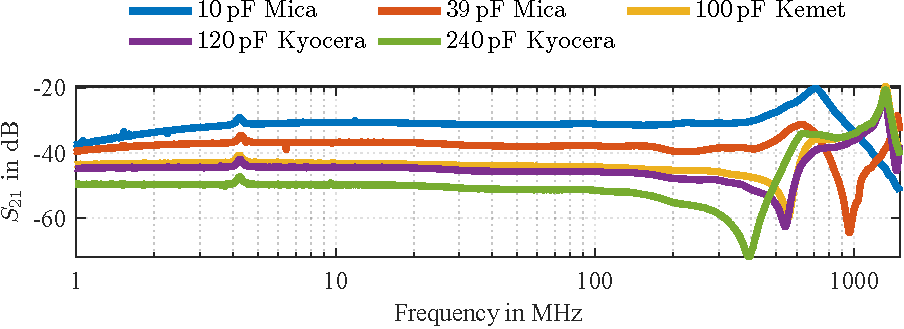
\includegraphics[scale=1]{figures/4_VoltageProbe/Voltage_Csense_Comp.pdf}
	\caption{Comparison of different sense capacitor technologies.}\label{fig:CapacitorComparison}
\end{figure}

In \fref{fig:CapacitorComparison}, the different capacitance values are reflected in the different transfer-function amplitudes.
Furthermore, the resonance frequency is visible where the transfer function shows a pole caused by the parasitic inductance of the sense capacitor.
This is summarized in \tref{tab:CapComp}, which shows the measured capacitance, the resonance frequency, and the calculated parasitic inductance.

\begin{table}
	\caption{Comparison of different high-frequency capacitor technologies.}
	\label{tab:CapComp}
	\centering
	\begin{tabular}{l l l l l}
		\toprule
		Manufacturer & Technology & Capacitance & Resonance Frequency & Calc. Inductance\\
		\midrule
		{Illinois} {Capacitor} & Mica & \SI{10}{pF} & -- & -- \\
		{Illinois} {Capacitor} & Mica & \SI{39}{pF} & \SI{956}{MHz} & \SI{710}{pH} \\
		Kemet & MLCC & \SI{100}{pF} & \SI{555}{MHz} & \SI{822}{pH} \\
		Kyocera & MLCC & \SI{120}{pF} & \SI{540}{MHz} & \SI{723}{pH} \\
		Kyocera & MLCC & \SI{240}{pF} & \SI{393}{MHz} & \SI{683}{pH} \\
		\bottomrule
	\end{tabular}
\end{table}

All technologies show a similar parasitic inductance, which is in the range of \SI{700}{pH} to \SI{800}{pH}.
This suggests that the parasitic inductance is determined not by the capacitor technology but by the package size, which is the same for all of them: a standard 0805 package.

The goal is to achieve a maximum sense capacitance, while keeping the resonance pole well above \SI{500}{MHz}, which is the targeted bandwidth of the probe.

A classical approach to increase the capacitance, without decreasing resonance frequency, is to connect multiple capacitors in parallel, which is done for the \SI{39}{pF} mica capacitor shown in \fref{fig:CsenseParallel}.
Here, the expectation is that the capacitance value increases by the number of parallel capacitors, while the parasitic inductance decreases by the same factor, resulting in a constant resonance frequency.
However, the measurement results show that the resonance frequency decreases with an increasing number of capacitors, caused by the remaining parasitic inductance of the PCB traces between the parallel-connected capacitors.

\begin{figure}[ht]
	\centering
	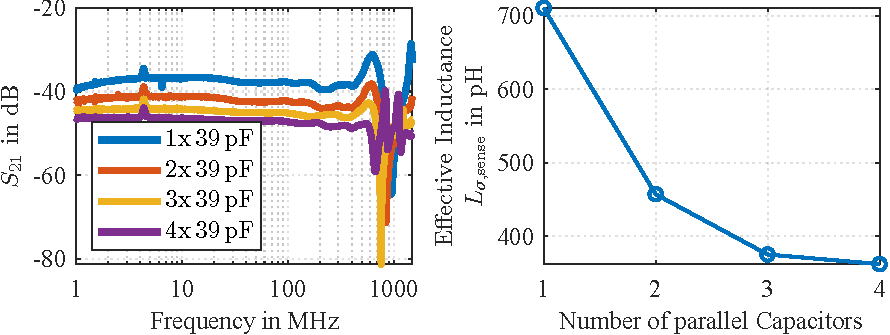
\includegraphics[scale=1]{figures/4_VoltageProbe/Voltage_Csense_parallel.pdf}
	\caption{Behavior of parallel-connected sense mica capacitors.}\label{fig:CsenseParallel}
\end{figure}

As can be seen, a maximum number of four capacitors can be connected in parallel, which results in a total capacitance of \SI{156}{pF} and a resonance frequency of \SI{670}{MHz}, which is the targeted bandwidth of the probe.
In \fref{fig:CsenseParallel} also the calculated parasitic inductance is plotted; for a number of four parallel capacitors, the parasitic inductance has only reduced by a factor of 1.9.




\textbf{High-Voltage Capacitor \mi{C}{HV}:} 
After the selection of the sense capacitor, the high-voltage capacitor \mi{C}{HV} is designed to achieve the desired divider ratio of \eref{eq:divider_ratio}.
Here, the high-voltage capacitor is the remaining part of the high-voltage capacitance, which is necessary to achieve the desired divider ratio, which is not created by the parasitic capacitance \mi{C}{\sigma 1,HV} of the high-voltage resistor \mi{R}{HV}, see \fref{fig:VoltageDividerPCB_parESB}.

\begin{figure}[ht]
	\centering
	\import{./figures/4_VoltageProbe/}{Diss_VoltageDividerPCB_Querschnitt.pdf_tex}
	\caption{Cross-section of the redesigned dual-channel differential active voltage probe PCB.}\label{fig:VoltageDividerPCB}
\end{figure}

It can be calculated as:
\begin{equation}
	\mi{C}{HV} = \frac{\mi{C}{sens}}{\mi{a}{CR}} - \mi{C}{\sigma 1,HV}.
\end{equation}
Given the lack of high-voltage, high-frequency capacitor technologies, a custom PCB-integrated parallel-plate capacitor was implemented. 
The capacitor is realized symmetrically: the positive signal path employs the copper layers between the top and second PCB layer, while the negative signal path utilizes the corresponding layers between the bottom and fifth PCB layer. 
This symmetric implementation ensures balanced performance across both differential channels.
Its capacitance can be calculated using the classical parallel-plate capacitor formula:
\begin{equation}
	\mi{C}{HV} = \frac{\varepsilon_0 \cdot \varepsilon_r \cdot A}{d},
\end{equation}
Since both the parasitic capacitance \mi{C}{\sigma 1,HV} of the high-voltage resistor and the prepreg width of the PCB have significant tolerances, the effective electrode area of the PCB capacitor is designed to be trimmable by adjusting the overlap of the top and bottom copper layers.
This is realized by the finger layout of the polygon, which can be seen in \fref{fig:VoltageDividerPCB_Polygon}.

\begin{figure}[ht]
	\centering
	\import{./figures/4_VoltageProbe/}{Diss_VoltageDividerPCB_Polygons.pdf_tex}
	\caption{Finger layout of the trimmable PCB capacitor.}\label{fig:VoltageDividerPCB_Polygon}
\end{figure}

\textbf{High-Voltage Resistor \mi{R}{HV} and Sense Resistor \mi{R}{sens}:} 
The resistor choice has only secondary importance for this work, since the main focus of this work is the high-frequency behavior of the probe, which is mainly defined by the capacitive elements of the voltage divider.
The cut-off frequency of the voltage divider is defined by the RC time constant of the high-voltage resistor \mi{R}{HV} and the sense capacitor \mi{C}{sens}, which is given by
\begin{align}	
	\mi{f}{c} &= \frac{1}{2\pi \cdot \mi{R}{HV} \cdot \mi{C}{HV}} \\
				&= \frac{1}{2\pi \cdot \SI{2}{M\Omega} \cdot \SI{0.2}{pF}} = \SI{500}{kHz}	
\end{align}

For the high-voltage resistor \mi{R}{HV}, a rather low resistance value was chosen in contrast to commercially available high-voltage probes, which typically use a \SI{10}{M\Omega} resistor.
This is done due to problems with the parasitic capacitance \mi{C}{\sigma 2,HV} of the high-voltage resistor, which causes time constants in the relevant frequency regime.
This was reduced by choosing a smaller resistor value, changing the resistor technology from a thick-film resistor to a thin-film resistor, and by creating a PCB cutout region just below the resistor, see \fref{fig:VoltageDividerPCB_Polygon}.

\textbf{Shielding:} 
In a previous version, the probe consisted of a four-layer PCB, which caused cross-coupling from the positive to the negative side and vice versa through the parasitic capacitance \mi{C}{\sigma 2,sens}.
This can be reduced by adding an additional shielding layer between the positive and negative signal path, which is implemented in a six-layer PCB, see \fref{fig:VoltageDividerPCB}.













\subsubsection*{Unity-Gain Amplifier}
The output of the voltage divider exhibits an impedance that varies with frequency due to the sense capacitance.
To achieve a constant output impedance over frequency, a unity-gain stage is implemented.
This unity-gain amplifier must have low noise, high bandwidth, and high input impedance to avoid loading the voltage divider and to maintain signal integrity.
Furthermore, for classical analysis such as overshoot, \sddt{v}, and \mi{e}{sw}, an accurate DC measurement is required.



A composite loop amplifier architecture was selected for the probe's unity-gain buffer to achieve both high DC precision and a wide bandwidth, a combination that is challenging to attain with a single amplifier. 
Precision operational amplifiers offer excellent DC accuracy (low offset and drift) but have limited gain-bandwidth products. 
Conversely, high-speed buffers provide multi-gigahertz bandwidth and high slew rates but typically have poorer DC characteristics. 
The composite loop topology leverages the strengths of two different amplifiers by creating separate signal paths for low-frequency and high-frequency signal components, which are then seamlessly recombined at the output.
The chosen composite loop amplifier architecture is depicted in \fref{fig:EME_ESB_UG}, where the low-frequency path is handled by a precision operational amplifier, while the high-frequency path is managed by a high-speed buffer.

\begin{figure}[ht]
	\centering
	\import{./figures/4_VoltageProbe/}{Diss_UnityGain_EME_ESB.pdf_tex}
	\caption{Equivalent circuit diagram of the unity-gain stage, which is designed as a composite loop amplifier.}\label{fig:EME_ESB_UG}
\end{figure}

\begin{table}[ht]
	\caption{Parameter values of the unity-gain amplifier}
	\centering
	\begin{tabular}[t]{l l}
		\toprule
		\textbf{Parameter} & \textbf{Value}\\
		\midrule
		\mti{OP}{1} & BUF802 			\\
		\mi{R}{1} & \SI{52.2}{k\Omega}	\\
		\mi{R}{3} & \SI{30}{\Omega}		\\		
		\mi{R}{5} & \SI{10}{k\Omega}	\\
		\mi{R}{8} & \SI{10}{\Omega}		\\
		\mi{C}{1} & n.p. 				\\
		\mi{C}{3} & \SI{27}{pF}			\\
		\bottomrule
	\end{tabular}
	\hspace{1cm}
	\begin{tabular}[t]{l l}
		\toprule
		\textbf{Parameter} & \textbf{Value}\\
		\midrule
		\mti{OP}{2} & OPA140 \\
		\mi{R}{2} & \SI{11}{k\Omega} \\
		\mi{R}{4} & \SI{2.44}{k\Omega} \\
		\mi{R}{6} & \SI{2}{k\Omega} \\
		\mi{R}{9} & \SI{80}{k\Omega}\\
		\mi{C}{2}  & \SI{270}{pF} \\
		\mi{C}{4} & \SI{100}{pF} \\
		\bottomrule
	\end{tabular}
\end{table}

The input signal is split into two paths using a frequency-dependent network.
A series capacitor \mi{C}{2} and a resistor \mi{R}{3} on the input of the high frequency OP \mti{OP}{1} form a high-pass filter. 
This directs high-frequency signals to the fast buffer path with the open loop gain $G$. 
The precision amplifier \mti{OP}{2} handles the signal for the auxiliary path, which dominates the low-frequency response. 

To ensure a flat frequency response across the crossover region where both amplifiers are active, the gain of the low-frequency path must precisely match the gain of the high-frequency path. 
The datasheet specifies the condition 
\begin{align}
	\sfrac{\alpha}{\beta} &= G \\
	\alpha &= \frac{\mi{R}{2}}{\mi{R}{1} + \mi{R}{2}}  \\
	\beta &= \frac{\mi{R}{4}}{\mi{R}{4} + \mi{R}{5}}
\end{align}

where $\alpha$ is the input attenuation factor of the precision amplifier path, and $\beta$ is the feedback factor of the precision amplifier.
Since the gain $G$ can vary between devices, the precision amplifier's feedback network must be trimmed during commissioning.

Lastly, the same gain must be achieved for the positive and negative unity-gain amplifiers.
This differs from device to device and is additionally affected by the different loading of the two unity-gain stages, due to the asymmetrical load of the subtractor, which is connected to the output of the unity-gain amplifier.
To still achieve the same gain for both unity-gain amplifiers, a voltage divider formed by \mi{R}{8} and \mi{R}{9} is implemented, which must be trimmed during commissioning.
Any asymmetry in the gain of the unity-gain amplifiers would lead to a non-zero output of the subtractor, which directly worsens the CMRR.


\begin{figure}[ht]
	\centering
	\input{"figures/4_VoltageProbe/VNA_rawUG.tex"}
	\caption{VNA measurement of the unity-gain amplifier.}\label{fig:VNA_rawUG}
\end{figure}

\subsubsection*{Dual-Channel Subtractor}
Up to this point, the probe design is similar to conventional differential probes, which typically employ a single subtractor stage to generate the differential output signal.
However, now the signal is split into two separate paths, each with its own dedicated subtractor stage.
The low-pass -- or conventional -- subtractor amplifier is designed to provide a flat frequency response up to the frequency where the signal falls below the noise floor (normally around \SI{120}{MHz}).
The high-pass subtractor amplifier is designed to provide a frequency response of \SI{+40}{dB/dec} to enable an analysis of the EMC-relevant frequency range, as discussed in Chapter \ref{ch:Methods}.

\subsubsection*{Low-Pass Subtractor}
The equivalent circuit diagram of the low-pass subtractor is shown in \fref{fig:EME_ESB_LP} and its used parameter values in \tref{tab:ComponentsLowPass_Voltage}.

\begin{figure}[ht]
	\centering
	\import{./figures/4_VoltageProbe/}{Diss_Lowpass_EME_ESB.pdf_tex}
	\caption{Equivalent circuit diagram of the low-pass subtractor.}\label{fig:EME_ESB_LP}
\end{figure}

\begin{table}[ht]
	\caption{Parameter values of the low-pass subtractor.}
	\label{tab:ComponentsLowPass_Voltage}
	\centering
	\begin{tabular}[t]{l l}
		\toprule
		\textbf{Parameter} & \textbf{Value}\\
		\midrule
		\mti{OP}{LP} & OPA817 		\\
		\mi{R}{10} & \SI{180}{\Omega}\\
		\mi{R}{11} & \SI{180}{\Omega}\\		
		\mi{R}{12} & \SI{180}{\Omega}\\
		\bottomrule
	\end{tabular}
	\hspace{1cm}
	\begin{tabular}[t]{l l}
		\toprule
		\textbf{Parameter} & \textbf{Value}\\
		\midrule
		\mi{R}{13} & \SI{180}{\Omega}\\
		\mi{R}{14} & \SI{10}{\Omega} \\
		\mi{C}{5} & n.p.			 \\
		\mi{C}{6} & n.p.			 \\
		\bottomrule
	\end{tabular}
\end{table}

The circuit follows a classical differential amplifier topology, where the output voltage is given by
\begin{equation}
	\mi{v}{LP} = \mi{v}{UG+}\cdot\frac{\mi{R}{11}}{\mi{R}{10}+\mi{R}{11}}\left(\frac{\mi{R}{12}}{\mi{R}{12}+\mi{R}{13}}\right) - \mi{v}{UG-}\cdot\frac{\mi{R}{13}}{\mi{R}{12}} \\
\end{equation}
which simplifies for a symmetric design of the resistors $\mi{R}{10} = \mi{R}{12}$ and $\mi{R}{11} = \mi{R}{13}$
\begin{equation}
	\mi{v}{LP} = \frac{\mi{R}{11}}{\mi{R}{10}} \cdot (\mi{v}{UG+} - \mi{v}{UG-})
\end{equation}

If a defined cut-off frequency is desired, the output can be low-pass filtered by adding capacitors \mi{C}{5} and \mi{C}{6} in parallel to the feedback resistors \mi{R}{13} and \mi{R}{14}, respectively.
However, in the current design, these capacitors are not populated, and the roll-off is defined by the operational amplifier.

\begin{figure}[ht]
	\centering
	\input{"figures/4_VoltageProbe/VNA_rawLP.tex"}
	\caption{VNA measurement of the low-pass subtractor.}\label{fig:VNA_rawLP}
\end{figure}

\subsubsection*{High-Pass Subtractor}
The high-pass subtractor is designed to provide a frequency response of \SI{+40}{dB/dec} to enable an analysis of the EMC-relevant frequency range, as discussed in Chapter \ref{ch:Methods}.
The equivalent circuit diagram of the high-pass subtractor is shown in \fref{fig:EME_ESB_HP} and its used parameter values in \tref{tab:ComponentsHighPass_Voltage}.

\begin{figure}[ht]
	\centering
	\import{./figures/4_VoltageProbe/}{Diss_Highpass_EME_ESB.pdf_tex}
	\caption{Equivalent circuit diagram of the high-pass filter.}\label{fig:EME_ESB_HP}
\end{figure}

\begin{table}[ht]
	\caption{Parameter values of the high-pass subtractor.}
	\label{tab:ComponentsHighPass_Voltage}
	\centering
	\begin{tabular}[t]{l l}
		\toprule
		\textbf{Parameter} & \textbf{Value}\\
		\midrule
		\mti{OP}{HP1} & LMH5401 		\\
		\mi{C}{7}, \mi{C}{8} & \SI{6}{pF}\\
		\mi{R}{15}, \mi{R}{16} & \SI{10}{\Omega}\\
		\mi{R}{17}, \mi{R}{18} & \SI{400}{\Omega}\\	
		\mi{R}{fb} & \SI{25}{\Omega}\\
		\mi{R}{out} & \SI{10}{\Omega}\\
		\mi{R}{19},\mi{R}{20} & \SI{10}{\Omega}\\
		\bottomrule
	\end{tabular}
	\hspace{0.5cm}
	\begin{tabular}[t]{l l}
		\toprule
		\textbf{Parameter} & \textbf{Value}\\
		\midrule
		\mti{OP}{HP2} & LMH5401 		\\
		\mi{C}{9}, \mi{C}{10} & \SI{6}{pF}\\
		\mi{R}{21}, \mi{R}{22} & \SI{10}{\Omega}\\		
		\mi{R}{23}, \mi{R}{24} & \SI{200}{\Omega}\\		
		\mi{R}{fb} & \SI{25}{\Omega}\\
		\mi{R}{out} & \SI{10}{\Omega}\\
		\mi{R}{25}, \mi{R}{26} & \SI{10}{\Omega}\\
		\bottomrule
	\end{tabular}
	\hspace{0.5cm}
	\begin{tabular}[t]{l l}
		\toprule
		\textbf{Parameter} & \textbf{Value}\\
		\midrule
		\mti{OP}{HP3} & THS4302\\
		\mi{R}{27} & \SI{50}{\Omega}\\		
		\mi{R}{28} & \SI{200}{\Omega}\\
		\mi{R}{g} & \SI{50}{\Omega}\\		
		\mi{R}{f} & \SI{200}{\Omega}\\	
		\mi{R}{29} & \SI{10}{\Omega}\\
		\bottomrule
	\end{tabular}
\end{table}

The high-pass subtractor uses a cascaded design.
The gain can be calculated as
\begin{equation}
	\mi{v}{HP} = \mi{G}{HP1} \cdot \mi{G}{HP2} \cdot \mi{G}{HP3} \cdot (\mi{v}{UG+} - \mi{v}{UG-})
\end{equation}
with
\begin{align}
	\mi{G}{HP1} &= \frac{s\omega \mi{C}{7}(\mi{R}{17}+ \mi{R}{fb})}{s\omega \mi{C}{7}\mi{R}{15}+1}\\
	\mi{G}{HP2} &= \frac{s\omega \mi{C}{9}(\mi{R}{23}+ \mi{R}{fb})}{s\omega \mi{C}{9}\mi{R}{21}+1}\\
	\mi{G}{HP3} &= \frac{\mi{R}{f}}{\mi{R}{g}}
\end{align}

again, for total symmetry between the positive and negative signal paths, the same component values are used for both channels.
	

Although a second-order high-pass response could in principle be realized with a single stage, this would result in increased signal attenuation due to the additional high-pass impedance.
Since the voltage divider already introduces a large attenuation, compensating gain is required to raise the signal to a level suitable for the oscilloscope input while keeping it well above the oscilloscope's noise floor.
This represents a careful design trade-off: increasing the gain of the secondary amplifier stage also amplifies its noise contribution, potentially degrading the overall signal-to-noise ratio.
Following Friis' noise formula for cascaded systems, the noise figure of the chain is governed by
\begin{equation}
	\mi{F}{total} = \mi{F}{1} + \frac{\mi{F}{2}-1}{\mi{G}{1}} + \frac{\mi{F}{3}-1}{\mi{G}{1}\cdot\mi{G}{2}} + \cdots
\end{equation}
which shows that the first stage dominates the overall noise performance.
Consequently, the first stage carries the highest gain, while the second stage contributes only the additional filter order required to achieve the desired \SI{+40}{dB/dec} slope.
The final stage converts the differential signal to a single-ended output; using only one of the two differential outputs was also evaluated but resulted in a lower SNR.


\begin{figure}[ht]
	\centering
	\input{"figures/4_VoltageProbe/VNA_rawHP.tex"}
	\caption{VNA measurement of the high-pass subtractor.}\label{fig:VNA_rawHP}
% TODO: measurement must be repeated
\end{figure}

Figure~\ref{fig:VNA_rawHP} shows the measured frequency response of the high-pass subtractor, which confirms the expected \SI{+40}{dB/dec} slope up to the cutoff-frequency of the high-pass at \SI{400}{MHz}.
At the cutoff frequency, the final gain is \SI{27}{dB}.

\subsubsection*{Shielding Concept and Implementation}

The last part of the probe required for a fully functional design is the shielding concept, which is necessary to avoid parasitic coupling between the probe and its environment in both directions.
Here, the main noise source is the switching node potential, which is in close proximity to the probe and, hence, is susceptible to capacitive couplings.

Therefore, the probe is shielded by a metal housing, which is connected to the analog ground potential and, thereby, to the oscilloscope ground.
A photograph of the housing is depicted in \fref{fig:Pic_EMEProbe}.
The high-voltage and active amplification circuitry are shielded separately; however, to avoid ground loops, they are manufactured as a single aluminum block, which is milled to create the necessary cavities for the functional blocks.

% TODO: add measurement with and without shielding.


%!TeX root = main.tex
%!encoding = UTF-8 Unicode

\subsection{Verification}
This section provides a rigorous verification of the dual-channel differential active voltage probe.
This probe enables access to high-frequency drain-source voltage components that are not reliably captured by conventional probe solutions; therefore, verification is treated as a central requirement rather than a supplementary step.
Accordingly, a comprehensive set of verification measurements is conducted to demonstrate that the relevant error mechanisms introduced in Section~\ref{sec:fundamental_measurement_errors} do not materially distort the reported results.

The updated probe was validated using the methodology of~\cite{kragl_active_2025}: small-signal characterization with a vector network analyzer (VNA), large-signal verification with a \SI{50}{\ohm} pulse generator, and low-pass cross-verification against a standard passive probe to exclude unintended capacitive or inductive coupling into the active measurement path.









\textbf{Small-Signal Verification for Differential Probes:}
The first test is a small-signal verification using a VNA to measure the frequency response of both the low-pass and high-pass channels.
The VNA was calibrated using an Open-Short-Load procedure at the probe input, with the VNA source impedance set to \SI{50}{\Omega}.
Measurements focus on the magnitude response to validate gain flatness for the low-pass channel and to verify bandwidth performance for both channels.

Since the probe is designed for differential operation but only a two-port VNA is available, the measurement is conducted in two separate single-ended configurations, as illustrated in \fref{fig:EME_VNA_SchematicOverview}.
The shared ground potential of the two VNA ports effectively shorts the differential input not under test, so only one input path can be characterized at a time.
The measurement is therefore repeated with the positive and negative differential inputs swapped, yielding the frequency response for both signal paths individually.
Comparing the two results also reveals the degree of input symmetry, which is directly relevant to the probe's common-mode rejection ratio (CMRR).

\begin{figure}[ht]
	\centering
	\import{./figures/4_VoltageProbe/}{Diss_SchematicOverview_EME_VNA.pdf_tex}
	\caption{Small-signal verification setup: single-ended VNA measurement of one differential input at a time. The VNA ground connection shorts the inactive differential input; the measurement is repeated with swapped connections to characterize both input paths.}\label{fig:EME_VNA_SchematicOverview}
\end{figure}

The design targets are a bandwidth exceeding \SI{120}{MHz} for the low-pass channel (where the noise floor typically emerges in power electronics measurements) and \SI{500}{MHz} for the high-pass channel.

The VNA results for the low-pass and high-pass channels are shown in \fref{fig:VNA_LP} and \fref{fig:VNA_HP}, respectively.
Here both differential inputs are measured, where the positive signal path is plotted with a solid line and the negative signal path with a dashed line.
Additionally, the measurement was executed with \SI{0}{dBm} input power for the positive and \SI{-10}{dBm} for the negative input.
This can be seen in the corresponding different noise floors at \SI{-100}{dB} and \SI{-80}{dB} for the positive and negative input of \mti{S}{11,LP}, respectively.

\begin{figure}[ht]
	\centering
	\input{"figures/4_VoltageProbe/VNA_LP.tex"}
	\caption{VNA measurement of positive (LPp) and negative (LPn) low-pass paths, crosscheck~\fref{fig:EME_VNA_SchematicOverview}.}\label{fig:VNA_LP}
\end{figure}

From this measurement also the probe voltage gain \mti{a}{probe} is obtained from the S-parameter measurement as
\begin{align}
	\mti{a}{probe} 	&= \frac{\mi{v}{out}}{\mi{v}{HV+}-\mi{v}{HV-}} \\
					&= \frac{\mti{S}{21}}{1 + \mti{S}{11}}.
\label{eq:TF_probe}
\end{align}

Since \mti{S}{11} remains nearly constant because of the probe's high input impedance, \mti{S}{21} is the dominant parameter for gain evaluation.
This expression holds under the assumption of equal gain in both differential input paths, a condition verified by the symmetry measurements described above.
In the presence of a gain mismatch, the effective transfer function would depend on the common-mode voltage partitioning between the two inputs — determined by the oscilloscope ground potential relative to the drain-source midpoint — a quantity that is generally undefined during in-circuit measurements.

The low-pass channel exhibits a flat passband gain of \SI{-53}{dB}, corresponding to a voltage division ratio of 446, in close agreement with the voltage divider design value.
The gain remains flat across the passband and rolls off at a \SI{3}{dB} bandwidth of \SI{315}{MHz}, primarily limited by the low-pass subtractor operational amplifier (see \fref{fig:VNA_rawLP}).
This substantially exceeds the design target of \SI{120}{MHz}, providing ample margin across the frequency range relevant to power electronics measurements.
The two input paths show close gain agreement, with a maximum deviation of \SI{0.2}{dB} at \SI{3}{MHz}, confirming the high degree of symmetry required for accurate differential measurements.

The high-pass channel, shown in \fref{fig:VNA_HP}, exhibits a gain slope of approximately \SI{+40}{dB/dec} from \SI{1}{MHz} to \SI{450}{MHz}, beyond which the unity-gain output amplifier begins to roll off.
The input-path gain deviation remains below \SI{0.8}{dB} within the linear-gain region, but increases to \SI{2.8}{dB} at \SI{490}{MHz} as both paths approach their respective rolloff frequencies.
The \SI{3}{dB} bandwidth exceeds the \SI{400}{MHz} lower design target, confirming that the channel adequately resolves high-frequency switching harmonics.
For measurements extending to \SI{500}{MHz}, the growing input-path gain mismatch must be considered, as it introduces an increasing common-mode error in the differential result.

\begin{figure}[ht]
	\centering
	\input{"figures/4_VoltageProbe/VNA_HP.tex"}
	\caption{VNA measurement of positive (HPp) and negative (HPn) high-pass paths, crosscheck~\fref{fig:EME_VNA_SchematicOverview}.}\label{fig:VNA_HP}
\end{figure}

In both measurements, a pole of the voltage divider is apparent at \SI{695}{MHz}, attributed to the RC network that establishes the probe input impedance.

\mti{S}{22} confirms the \SI{10}{\Omega} output resistance in both channels, consistent with the design specification for use with appropriate attenuators in \SI{50}{\Omega} measurement systems.
\mti{S}{11} reflects the high-impedance input of the voltage divider, yielding an approximately \SI{0}{dB} reflection coefficient and confirming negligible loading on the circuit under test.
\mti{S}{12} reveals a residual passive coupling path from output to input; however, this reverse transmission remains sufficiently small that it does not materially affect measurement accuracy within the verified frequency range.













\textbf{Large-Signal Verification with High-Voltage \SI{50}{\Omega} Pulse Generator:}
In addition to the small-signal VNA characterization, the probe was validated by a large-signal measurement using a \SI{400}{V}, \SI{50}{\ohm} pulse generator.
The schematic of the measurement setup is shown in \fref{fig:MS_PulsGen_SchematicOverview}.

\begin{figure}[ht]
	\centering
	\import{./figures/4_VoltageProbe/}{Diss_PulseGenerator_ESB.pdf_tex}
	\caption{Large-signal verification of the low-pass and high-pass channels using a \SI{50}{\ohm} pulse generator~\cite{kragl_active_2025}. The reference is acquired both via a conventional direct measurement and through a commercial \SI{180}{MHz}--\SI{340}{MHz} passive band-pass filter.}\label{fig:MS_PulsGen_ESB}
\end{figure}

This setup provides a well-characterized reference voltage signal attenuated by \SI{40}{dB} through a \SI{50}{\Omega} resistor, enabling direct connection to the oscilloscope without additional impedance mismatch.
The measurement system bandwidth is determined by the oscilloscope (\SI{2}{GHz}), which is sufficient to resolve transients in the millisecond to sub-microsecond range.
A photograph of the measurement setup is shown in \fref{fig:MS_PulsGen_Pic}.

\begin{figure}[ht]
	\centering
	\import{./figures/4_VoltageProbe/}{Diss_PulseGenerator_Pic.pdf_tex}
	\caption{Large-signal verification of the low-pass and high-pass channels using a \SI{50}{\ohm} pulse generator~\cite{kragl_active_2025}. The reference is acquired both via a conventional direct measurement and through a commercial \SI{180}{MHz}--\SI{340}{MHz} passive band-pass filter.}\label{fig:MS_PulsGen_Pic}
\end{figure}

The pulse generator employs \SI{750}{V} GaN-HEMTs with the \SI{40}{dB} attenuator serving as the load, producing fast resistive switching transients with risetimes below \SI{10}{ns}.
This transient speed is critical for validating the probe's ability to capture high-frequency switching dynamics without significant slew-rate-induced errors.
The \SI{50}{\Omega} output impedance of the pulse generator also enables direct connection of commercial BNC band-pass filters, allowing independent verification of different frequency bands without the noise-limiting effects of broadband low-pass filtering.


\fref{fig:MS_PulsGen_TD} presents the time-domain measurement of the low-pass channel, comparing three signals: the attenuated pulse generator reference, a commercial passive high-voltage probe, and the DAVP low-pass channel.
The low-pass channel bandwidth (\SI{315}{MHz} from VNA measurements) is sufficient to capture the primary switching transient; however, a second-order transient response emerges during the tail, attributed to slew-rate limiting of the low-pass subtractor operational amplifier at signal levels exceeding \SI{2}{Vpp}.
The small-signal bandwidth of this op-amp (\SI{800}{MHz} at \SI{100}{mVpp}) degrades to \SI{250}{MHz} at \SI{2}{Vpp} and \SI{140}{MHz} at \SI{4}{Vpp} according to the datasheet.
In contrast, the shared unity-gain buffer amplifier (used by both channels) exhibits minimal slew-rate effects, with measured bandwidths of \SI{3.1}{GHz} at \SI{100}{mVpp} and \SI{1.6}{GHz} at \SI{2}{Vpp}.
The DAVP low-pass channel accurately captures the initial rising edge of the transient.
However, the PT2 behavior present in the transient tail introduces a waveform distortion that results in a settling time of around \SI{20}{ns} before the final value is reached.
Since this effect is confined to the low-pass subtractor amplifier, it does not affect the high-pass channel.


\begin{figure}[ht]
	\centering
	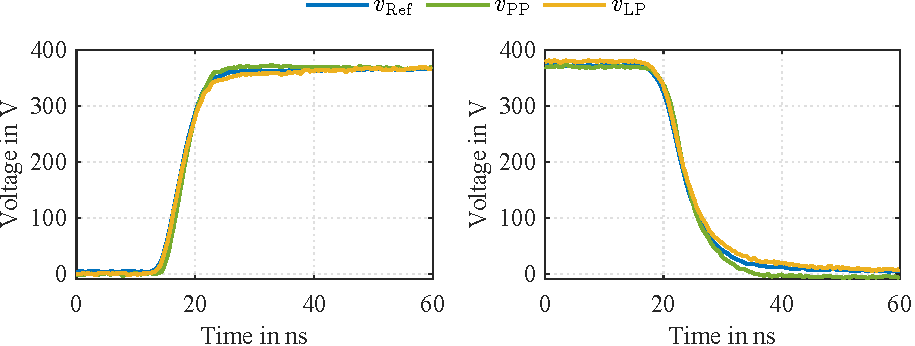
\includegraphics[scale=1]{figures/4_VoltageProbe/MS_PulsGen_TD.pdf}
	\caption{Large-signal verification time-domain of the low-pass using a \SI{50}{\ohm} pulse generator~\cite{kragl_active_2025}. The reference is acquired both via a conventional direct measurement and through a commercial \SI{180}{MHz}--\SI{340}{MHz} passive band-pass filter.}\label{fig:MS_PulsGen_TD}
\end{figure}

For high-pass channel verification, the pulse generator output is passed through a commercial \SI{180}{MHz}--\SI{340}{MHz} passive BNC band-pass filter, which isolates the high-frequency components while attenuating the DC and low-frequency content.
For this verification it is only useful to compare the calibrated frequency domain results, because the band-pass and the high-pass channel have completely different time-domain responses.
The frequency-domain results are shown in \fref{fig:MS_PulsGen_Meas}, comparing four traces: the unfiltered reference spectrum, the band-pass filtered reference spectrum, the low-pass channel spectrum, and the high-pass channel spectrum.
A sequence of pulses ensures matched quantization noise floors between the reference and measurement channels, enabling direct amplitude comparison.

\begin{figure}[ht]
	\centering
	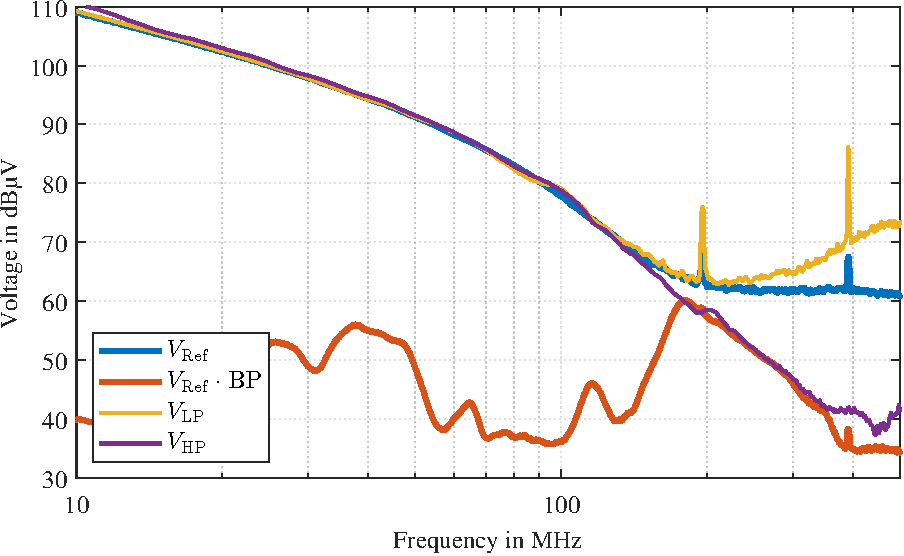
\includegraphics[scale=1]{figures/4_VoltageProbe/MS_PulsGen.pdf}
	\caption{Large-signal verification of the low-pass and high-pass channels using a \SI{50}{\ohm} pulse generator~\cite{kragl_active_2025}. The reference is acquired both via a conventional direct measurement and through a commercial \SI{180}{MHz}--\SI{340}{MHz} passive band-pass filter.}\label{fig:MS_PulsGen_Meas}
\end{figure}

At frequencies where the reference remains above the noise floor, the high-pass channel shows close agreement with both the reference and the low-pass channel, with a gradually increasing deviation below \SI{10}{MHz} as the high-pass channel attenuates the low-frequency content by design.
Within the band-pass filter passband (\SIrange{180}{340}{MHz}), the high-pass channel exhibits a maximum deviation of \SI{1.3}{dB} at \SI{200}{MHz}, with deviations below \SI{1}{dB} across most of the band.
Above \SI{340}{MHz}, independent verification is no longer possible, as no commercially available band-pass filter covers the \SIrange{300}{400}{MHz} region.
In this unverified range, the measured spectrum exhibits a plateau rather than the expected continuous rolloff, indicating a measurement artifact that may increase the error beyond \SI{1.3}{dB}.
Accordingly, results presented in the following analysis are shown up to \SI{500}{MHz}, but the probe is fully verified only up to \SI{340}{MHz}; results above this frequency should be interpreted as comparative rather than absolute calibrated values.


In summary, both channels satisfy their respective large-signal verification objectives.
The low-pass channel reliably captures the initial switching edge despite the slew-rate-induced PT2 behavior in the transient tail.
The high-pass channel demonstrates a maximum deviation of \SI{1.3}{dB} across the verified frequency range, consistent with the small-signal characterization results.
Together, these results confirm that the DAVP performs as designed under large-signal conditions relevant to power semiconductor measurements.











\textbf{Parasitic Couplings and Common-Mode Error:}

In a next verification step, the probe is assessed in the intended application environment by measuring the drain-source voltage of a SiC MOSFET during switching transients with both a commercial passive probe and the proposed DAVP.
The setup corresponds to the commutation cell used later in this work, operated in double-pulse mode with the actively switched device located in the low-side position.

The purpose of this measurement is twofold: first, to exclude unintended parasitic coupling paths introduced by the active probe; and second, to quantify the residual common-mode error under realistic switching conditions.
Both effects could distort the measured drain-source voltage and would therefore directly limit the interpretability of the later application measurements.
Because the passive reference probe is subject to the same quantization-noise limitations as all conventional measurements in the high-frequency region, the comparison is primarily performed in the time domain.
The corresponding results are shown in \fref{fig:Voltage_DPT_LPvsPP_weCM_TD} and \fref{fig:Voltage_DPT_HPvsPP_weCM_TD}.
For the dedicated common-mode measurement, both differential probe inputs are connected to the same potential, namely the source terminal of the MOSFET, so that the remaining output directly reflects the finite common-mode rejection of the probe.

\begin{figure}[ht]
	\centering
	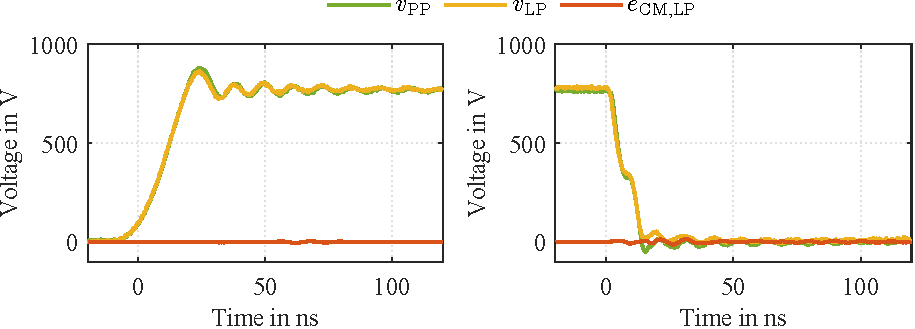
\includegraphics[scale=1]{figures/4_VoltageProbe/Voltage_DPT_LPvsPP_weCM_TD.pdf}
	\caption{Time-domain measurement results of PMTX05, at 800V, 30A room temperature, cross validation of passive probe and low-pass measurement to crosscheck inductive and capacitive coupling effects.}\label{fig:Voltage_DPT_LPvsPP_weCM_TD}
\end{figure}

The low-pass measurement again shows close agreement with the passive probe, indicating that the active probe does not introduce additional parasitic coupling paths that would materially distort the drain-source voltage waveform.
The remaining deviation is consistent with the limited large-signal settling behavior discussed previously and is most visible during the faster active-on transition, which exhibits a settling interval of approximately \SI{14}{ns}, compared with about \SI{32}{ns} during active-off switching.
The dedicated common-mode measurement furthermore shows that the residual common-mode error remains below \SI{4}{V} during active-off and below \SI{14}{V} during active-on, corresponding to less than \SI{1.8}{\percent} of the measured voltage.
These values confirm that common-mode feedthrough remains a secondary error source for the intended switching analysis.

Additionally, \fref{fig:Voltage_DPT_HPvsPP_weCM_TD} shows the time domain high-pass channel measurement with a differential and common-mode error measurement.
Here, also, only a small change is measured.

\begin{figure}[ht]
	\centering
	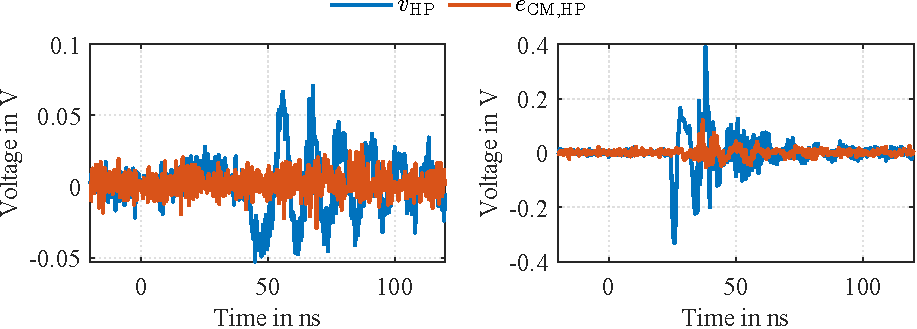
\includegraphics[scale=1]{figures/4_VoltageProbe/Voltage_DPT_HPvsPP_weCM_TD.pdf}
	\caption{Time-domain measurement results of PMTX05, at 800V, 30A room temperature, cross validation of passive probe and high-pass measurement to crosscheck inductive and capacitive coupling effects.}\label{fig:Voltage_DPT_HPvsPP_weCM_TD}
\end{figure}

To determine how much the shield of the probe influences the measurement, a measurement with and without the shield is performed, the results of which are shown in \fref{fig:Influence_Shield_TD} and \fref{fig:Influence_Shield_FD}.
The influence of the capacitive coupling becomes visible in the time domain, where the unshielded measurement shows a higher overshoot and ringing, which is also visible in the frequency domain, where the unshielded measurement shows a higher amplitude at higher frequencies.
Additionally, it can be seen that the shield is still not perfect, since the turned-on MOSFET still shows a small oscillation and offset, both of which should be zero in an ideal measurement.

\begin{figure}[ht]
	\centering
	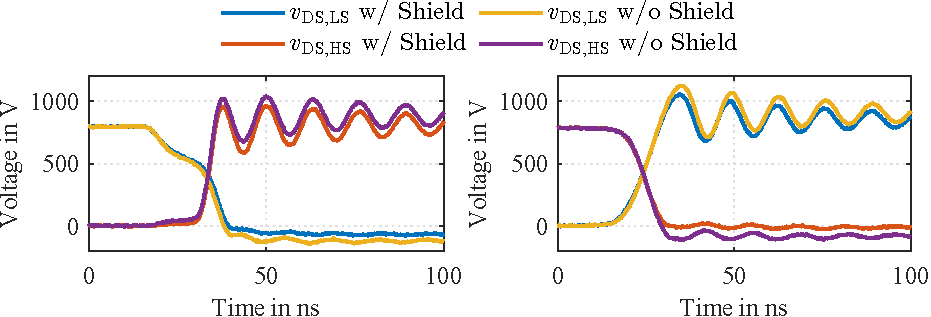
\includegraphics[scale=1]{figures/4_VoltageProbe/Influence_Shield_TD.pdf}
	\caption{Time-domain measurement results of PMTX05, at 800V, 30A room temperature, influence of the shield on the measurement.}\label{fig:Influence_Shield_TD}
\end{figure}

\begin{figure}[ht]
	\centering
	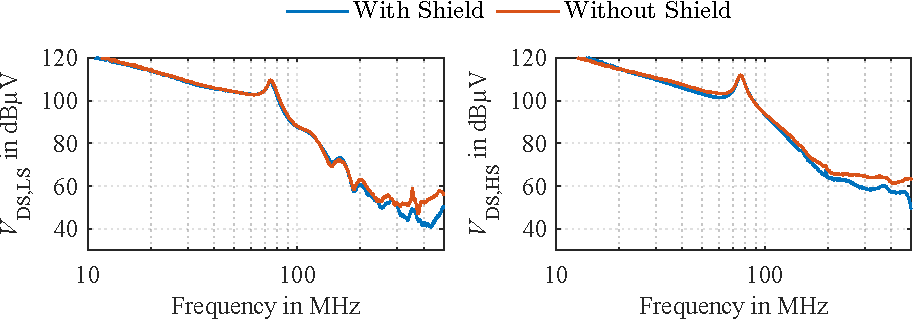
\includegraphics[scale=1]{figures/4_VoltageProbe/Influence_Shield_FD.pdf}
	\caption{Frequency-domain measurement results of PMTX05, at 800V, 30A room temperature, influence of the shield on the measurement.}\label{fig:Influence_Shield_FD}
\end{figure}


\textbf{Noise Performance Characterization:}
The final step of this section is not a strict verification, but rather a characterization of the probe's noise behavior.
This analysis clarifies the probe limitations and provides context for interpreting subsequent measurement results.


Figure~\ref{fig:Diss_Voltage_NoiseContribution} shows the frequency-domain noise behavior for an acquisition length corresponding to the pulse chain duration used later (\SI{5}{ms}).
First, the high-pass channel was measured at the oscilloscope resolution used for subsequent signal measurements (Probe + HV Resolution).
Second, a noise measurement was performed at the same resolution with the probe disconnected (HV Resolution).
Third, the measurement was repeated with the probe connected and full ADC resolution, which reduces quantization noise (Probe + Full Resolution).
Finally, a measurement without the probe and with full ADC resolution was performed to determine the oscilloscope noise floor (Full Resolution).

\begin{figure}[hbt]
	\centering
	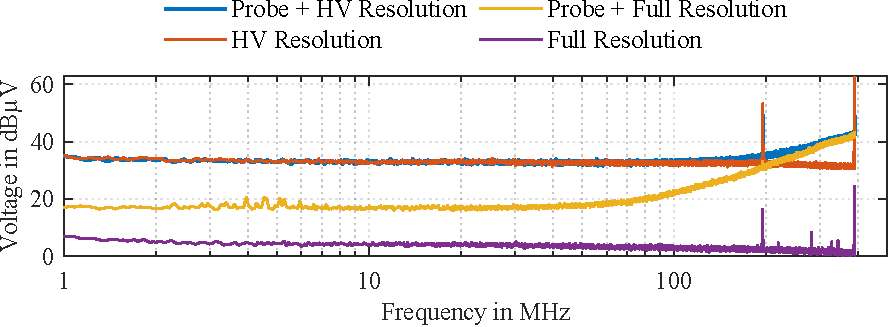
\includegraphics[scale=1]{figures/4_VoltageProbe/Diss_Voltage_NoiseContribution.pdf}
	\caption{Frequency domain measurement of the noise limiting effects of the EME voltage probe.}\label{fig:Diss_Voltage_NoiseContribution}
\end{figure}

Comparing the two no-probe measurements at different resolutions shows that quantization noise is the dominant contribution: the noise level decreases significantly from \SI{50}{dBµV} to \SI{22}{dBµV} when full ADC resolution is used.
With the probe connected, the intrinsic probe noise remains below the quantization-noise level of the HV-resolution measurement (\SI{33}{dBµV}) up to approximately \SI{100}{MHz}.
Above this frequency, the noise rises with the high-pass gain slope, which amplifies both signal and noise.
The crossover occurs at approximately \SI{200}{MHz}, beyond which intrinsic probe noise dominates over quantization noise.

Additionally, signal peaks can be seen at \SI{196}{MHz} and its harmonics.
This corresponds to the ADC interleaving frequency of the oscilloscope.
Interleaving is a technique used in oscilloscopes to increase the effective sampling frequency by operating multiple ADCs in parallel, each sampling at a fraction of the total rate.
Afterwards the signal is reconstructed by combining the outputs of the individual ADCs.
When not all ADCs are perfectly matched, this process can introduce spurious frequency components at the interleaving frequency and its harmonics, which is observed in the measurement.

\begin{figure}[hbt]
	\centering
	\import{./figures/4_VoltageProbe/}{Diss_Highpass_EME_NoiseSources_ESB.pdf_tex}
	\caption{Equivalent circuit diagram of the noise sources for the first high-pass amplification stage.}\label{fig:ESB_OP_noiseSources}
\end{figure}

To explain this behavior, an analytical noise calculation is performed for the second high-pass amplification stage.
Figure~\ref{fig:ESB_OP_noiseSources} shows the equivalent circuit of the noise sources in the high-pass amplifier, where \mi{Z}{g} is the series connection of the feedback capacitor and resistor.
Each resistor contributes Johnson–Nyquist thermal noise, while the capacitor itself does not generate thermal noise and only contributes through its equivalent series resistance (ESR).
The operational amplifier adds both input voltage noise and input current noise.

The relevant noise contributions are:
\begin{itemize}
	\item incoming noise from preceding stages,
	\item amplifier input voltage noise,
	\item resistor thermal noise,
	\item amplifier input current noise.
\end{itemize}

The resistor thermal noise is given by
\begin{equation}
	\mi{V}{n,th} = \sqrt{4\mi{k}{B}TR\Delta f}.
\end{equation}

The effective noise gain of the high-pass stage is
\begin{equation}
	 NG = 1 + \frac{\mi{R}{f}}{\mi{Z}{g}}.
\end{equation}

The total output noise can then be expressed as
\begin{equation}
	\mi{v}{0} = \sqrt{(\mi{v}{n,in} NG)^2 + (\mi{v}{n} NG)^2 + 2(\mi{i}{n} \mi{R}{f})^2 + 2\cdot4\mi{k}{B}T\mi{R}{f}\Delta f + 2\cdot4\mi{k}{B}T\mi{R}{g}\Delta f \left(\frac{\mi{R}{f}}{\mi{Z}{g}}\right)^2}.
\end{equation}

This formulation highlights that the amplifier noise is amplified by the noise gain, and that the noise response inherits the high-pass characteristic of the stage.

Figure~\ref{fig:Diss_Voltage_NoiseCalc} shows the calculated noise contributions using the datasheet values.
The dominant noise source at low frequency is the amplifier's input current noise, while at higher frequencies the input voltage noise becomes dominant.
Resistor thermal noise is negligible because the resistor values are only a few hundred \si{\ohm}.

The input noise of the previous stage follows the same trend: it is essentially the total noise of the first high-pass amplifier, multiplied by the noise gain of the second stage. 
The second cutoff at \SI{100}{MHz} is clearly visible where the noise changes from first to second order.


\begin{figure}[hbt]
	\centering
	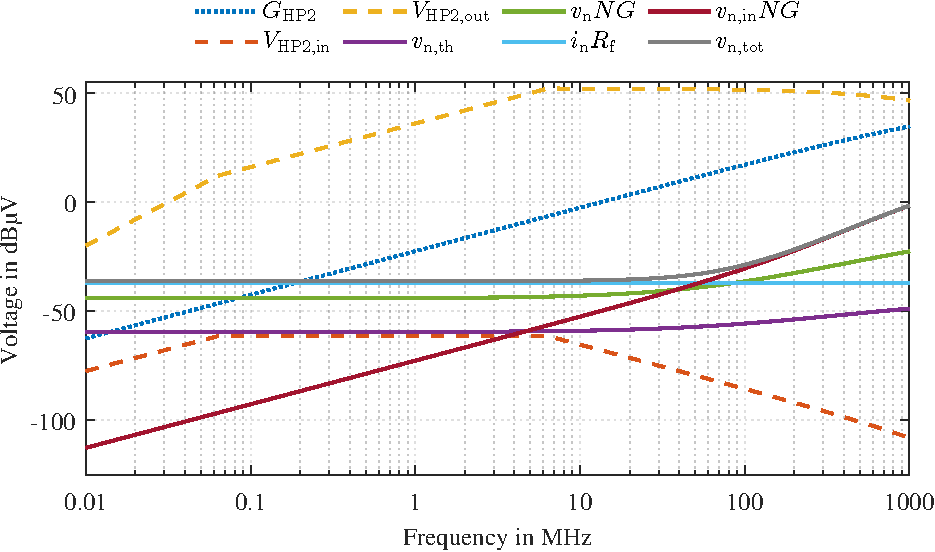
\includegraphics[scale=1]{figures/4_VoltageProbe/Diss_Voltage_Calc_Noise.pdf}
	\caption{Calculation of the noise sources for the first high-pass amplification stage.}\label{fig:Diss_Voltage_NoiseCalc}
\end{figure}


\section{Dual-Channel Active Current Probe}
\label{ch:AShunt}

While at lower frequencies the capacitive coupling from the switching node potential to the cooler dominates EMC concerns, recent studies indicate that inductive couplings become significant at higher frequencies as well~\cite{hamami_identifying_2026}.
Therefore, it is necessary to measure not only the high-frequency components of the voltage transient but also of the current transient.

%!TeX root = main.tex
%!encoding = UTF-8 Unicode

\subsection{Requirements for Broadband and Low-Intrusion Current Sensing}

Prior to designing the active current shunt, the measurement-driven requirements are defined.
As in the voltage-probe chapter, the requirements are derived from the EMC-relevant frequency range, practical measurement constraints, and expected disturbance mechanisms in the switching environment.
The aim is to obtain a current-sensing concept that does not materially disturb the commutation loop while still reproducing the frequency content relevant for EMC analysis.

\textbf{Small-Signal Response:}
The current-sensing path must provide a bandwidth of at least \SI{500}{MHz} to cover the EMC-relevant spectral content of the commutation current.
This bandwidth requirement excludes most commercial sensors, including Rogowski coils with usable bandwidths of approximately \SIrange{20}{50}{MHz}, magnetoresistive current sensors in the range of \SIrange{10}{100}{MHz}, and Hall-effect sensors in the range of \SIrange{1}{10}{MHz}~\cite{xin_review_2022}.
Bandwidths in the required range are only practical with shunt-based current sensing or with custom Rogowski-coil implementations using very few turns to minimize parasitic parameters.
Such Rogowski coils are, however, difficult to integrate robustly because their response is highly sensitive to positioning and orientation.
Therefore, a shunt-based approach is chosen for the current probe design.

\textbf{Large Signal Response:}
The large-signal requirement defines the maximum measurable current, i.e., the peak current amplitude the probe must handle without saturation or damage.
Unlike voltage, which is limited by a hard breakdown threshold of the device, the current limit of a MOSFET is a thermal constraint that depends on the duration of current flow.
During a switching transient, the instantaneous current can transiently exceed the nominal rated current of the device by a significant factor.
This is further exacerbated under high-temperature operating conditions, where bipolar degradation effects in SiC MOSFETs can lead to additional current peaks during the turn-off transient.

The upper current limit was therefore determined empirically based on measurements of the investigated devices under worst-case high-temperature conditions.
The device with the highest overcurrent under investigation is a \SI{60}{A} planar SiC MOSFET in a D2PAK package.
As shown in Section~\ref{sec:Results}, peak currents of up to \SI{140}{A} were observed, and accordingly the upper design limit was set to \SI{150}{A}.


\textbf{Loading and Measurement Intrusion:}
Shunt-based current measurement introduces a fundamental trade-off in EMC-oriented measurements.
The quality factor of the excited resonances is one of the main EMC-relevant characteristics of the switching transient, with the dominant resonance being formed by the commutation-loop inductance and the parasitic capacitances of the device under test.

The insertion of a shunt resistance into the commutation loop must therefore not materially alter the transient damping behavior.
As a rule of thumb, the inserted resistance should be at least one decade below the intrinsic damping resistance of the commutation cell.
For the present application, this value is dominated by the on-state resistance \mi{R}{DS,on} of the device under test.
For the considered \SI{750}{V} and \SI{1200}{V} discrete SiC devices in D2PAK, \mi{R}{DS,on} is in the range of \SIrange{20}{50}{m\ohm}~\cite{robert_bosch_gmbh_datasheet_2023,robert_bosch_gmbh_datasheet_2023-1}.
Accordingly, the sense resistance is limited to \SI{2}{m\ohm} or less.

This low resistance introduces a challenge for the achievable measurement bandwidth because each shunt exhibits parasitic inductance.
The resulting shunt bandwidth is

\begin{equation}
    \mi{f}{bw,shunt} = \frac{1}{2\pi \tau_\text{shunt}} = \frac{\mi{R}{shunt}}{2\pi\mi{L}{shunt}} 
    \label{eq:fbw_shunt}
\end{equation}

In classical shunt design, larger shunt resistance values support higher bandwidth.
This is shown in \fref{fig:Diss_Current_PassiveShuntCalc}, which illustrates the achievable bandwidth of a shunt with a parasitic inductance of \SI{250}{nH}, which is classical for a 0612 shunt package, as a function of the shunt resistance.
For the present EMC application, this trade-off cannot be exploited because the insertion resistance must remain very small.

\begin{figure}[ht]
	\centering
    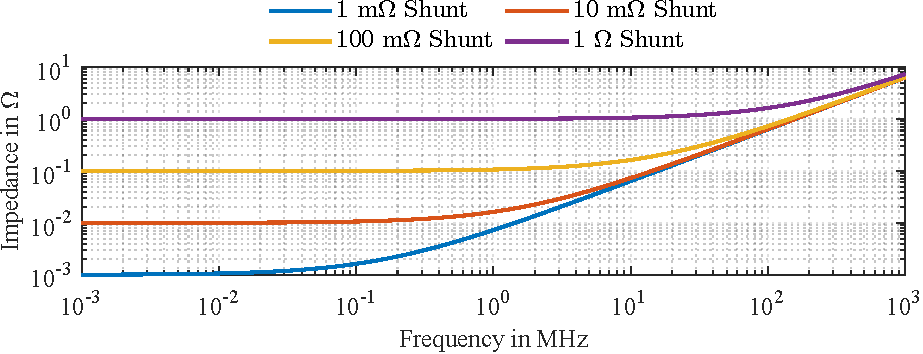
\includegraphics[scale=1]{figures/5_CurrentProbe/Diss_Current_PassiveShuntCalc.pdf}
	\caption{Achievable bandwidth of a passive current shunt with a parasitic inductance of \SI{250}{pH} as a function of the shunt resistance.}\label{fig:Diss_Current_PassiveShuntCalc}
\end{figure}

As can be seen in \fref{fig:Diss_Current_PassiveShuntCalc}, a passive shunt with a resistance of \SI{1}{m\ohm} and a parasitic inductance of \SI{250}{nH} would only achieve a bandwidth of approximately \SI{636}{kHz}.
However, to achieve a bandwidth of \SI{500}{MHz} for the given inductance, the resistance must be bigger than \SI{1}{\ohm}.
Options to further reduce the parasitic inductance of the shunt are limited by the physical size of the shunt and the required current-carrying capability.
The best passive shunt reported in the literature~\cite{wang_high_} achieved \SI{150}{pH} with a coaxial structure. 
However, for a resistance of \SI{2}{m\Omega}, this would still result in an insufficient bandwidth of \SI{2}{MHz}.


\textbf{Output Interface and Signal Routing:}
Analogous to the voltage-probe concept, the current probe must provide a \SI{50}{\Omega} output interface.
This is required to route the measured signal into both low-pass and high-pass processing paths with defined impedance conditions.
Consequently, a purely passive shunt implementation is not sufficient for the intended measurement chain.

\textbf{Isolation Requirement for Combined Measurements:}
For standalone current measurements, galvanic isolation is not mandatory because the probe can reference the oscilloscope ground.
However, for simultaneous measurements with LISN disturbance voltage, galvanic isolation becomes necessary because the oscilloscope ground is fixed to the aluminum base plate.
In this case, optical isolation of the measurement link is feasible and compatible with the required \SI{50}{\ohm} signal interface.


\textbf{Transmission Line Effects:}
As in the voltage-probe case, the interconnect between the shunt element and the subsequent measurement stage must be kept short enough to avoid transmission-line effects.
This applies to all non-\SI{50}{\ohm} interconnects, including the shunt element itself, the compensation amplifier, and the subsequent filter stage.
At the required bandwidth, any unnecessary cable length would introduce reflections and additional phase error, thereby distorting the measured current waveform.
This requirement is particularly relevant for the current shunt, whose resistance is in the \si{m\Omega} range.


\textbf{Parasitic Coupling:}
As for the voltage probe, parasitic coupling into the sensing path must be minimized.
For the active current shunt, parasitic coupling is particularly critical because the circuit is placed close to the switching node and operates with higher gain than the active voltage probe.


%!TeX root = main.tex
%!TeX root = main.tex
%!encoding = UTF-8 Unicode

\subsection{Probe Architecture and Implementation}

To meet the broadband, low-intrusion current sensing requirements defined in the previous section, an active current-shunt probe was designed. 
The core concept is to combine a passive shunt resistor with an active compensation amplifier, as shown in the simplified schematic in \fref{fig:ESBActiveShunt} and the prototype photograph in \fref{fig:ESBActiveShuntPhoto}.
The active shunt architecture consists of three main components: a passive shunt element, an active compensation stage, and a dual-channel filter stage.

\begin{figure}[htbp]
	\centering
	\tikzsetnextfilename{Diss_CompensatedCurrentShunt}
	\import{./figures/5_CurrentProbe/}{"Diss_CompensatedCurrentShunt.pdf_tex"}
	\caption{Simplified schematic overview of active current shunt.}\label{fig:ESBActiveShunt}
\end{figure}

This architecture offers multiple key advantages over a purely passive approach:

First, a small shunt resistance can be used while maintaining sufficiently high sense output voltage through operational amplifier gain, thereby reducing circuit loading and measurement intrusion on the device under test.

Second, the integrated compensation network addresses the high-pass roll-off inherent to passive shunt designs, enabling flat frequency response across the measurement bandwidth with usable range limited primarily by the operational amplifier's gain-bandwidth product.

Third, the amplified output signal enables flexible signal routing: either through a dual-channel filter network for simultaneous extraction of high-frequency EM noise and low-frequency power switching transients, or to an optically isolated measurement probe for galvanic isolation when required by system-level constraints.
This architecture is adapted from \cite{shillaber_gigahertz_2020,shillaber_ultrafast_2022} and tailored to the specific requirements of this application.

\begin{figure}[ht]
	\centering
	\import{./figures/5_CurrentProbe/}{"Diss_Pic_AShunt.pdf_tex"}
	\caption{Photograph of active current shunt.}\label{fig:ESBActiveShuntPhoto}
\end{figure}


The following subsections detail the design of the passive shunt element, the active compensation stage, and the integrated shielding approach.








\textbf{Passive Shunt Element and Layout Realization:}

The systematic layout of the passive shunt element is shown schematically in \fref{fig:ESBPassiveShunt}, with a photograph of the realized PCB provided in the same figure.

\begin{figure}[ht]
	\centering
	\tikzsetnextfilename{Diss_PassiveShuntPCB_3D_wSchematic}
	\import{./figures/5_CurrentProbe/}{"Diss_PassiveShuntPCB_3D_wSchematic.pdf_tex"}
	\caption{Design of passive part of the current shunt.}\label{fig:ESBPassiveShunt}
\end{figure}

\begin{table}[ht]
	\caption{Parameter values of the passive shunt element}
	\label{tab:ShuntParameters}
	\centering
	\begin{tabular}{ll}
		\toprule
		\textbf{Parameter} &  \textbf{Value} \\
		\midrule
		\mi{R}{shunt} & \SI{2}{m\Omega} \\
		\mi{L}{shunt} & \SI{24}{pH} \\
		\mi{G}{shunt} & \SI{2}{mV/A} \\
		\bottomrule
	\end{tabular}
\end{table}

The passive shunt element is realized using ten low-inductance, low-resistance shunt resistors in a 0508 package. 
These are metal foil resistors with a resistance of \SI{20}{m\ohm} each, which are connected in parallel to achieve a total resistance of \SI{2}{m\ohm}. 
The key advantage of metal foil resistors for this application is that they conduct their current on the bottom side of their package, which enables an optimal integration into a coplanar layout design.

The resistor placement strategy exploits this bottom-side current conduction to minimize parasitic inductance by maximising the mutual inductance.
This is realized through a half-circle placement on the PCB, with vias positioned on the outer edge. 
This geometry forces the return current to flow directly below the shunt resistors, minimizing loop area.
From the resistors, the return current is routed vertically to the DC link capacitors.

The layout approach is adapted from \cite{shillaber_gigahertz_2020}. 
However, in this application the parasitic inductance introduced by the measurement is less critical than in the reference design, since characterization is performed using the given commutation loop inductance \mi{L}{\sigma} without a specified minimum inductance target.

A surface-mount MMCX connector is incorporated into the design to enable measurement of the shunt's transfer function, which is essential for determining the compensating network values in the subsequent active compensation amplifier stage. 

The connection to the active amplification stage is routed through the two middle PCB layers, surrounded by a via fence connecting top and bottom ground planes for shielding. 
The ground reference used for this connection is the DC− potential of the DC link, distinct from the Kelvin source of the MOSFET under test. 



\textbf{Active Compensation for Bandwidth Extension and Impedance Matching:}
After the passive shunt element, the signal is routed to an active compensation stage.
This stage serves three functions: compensation of the shunt high-pass behavior caused by parasitic inductance, conversion of the shunt signal into a defined voltage signal, and provision of a \SI{50}{\ohm} output interface for subsequent measurement stages.

The schematic overview of the compensation stage is shown in \fref{fig:ESBCompensation}.

\begin{figure}[ht]
	\centering
	\tikzsetnextfilename{Diss_Compensation_Shunt_ESB}
	\import{./figures/5_CurrentProbe/}{"Diss_Compensation_Shunt_ESB.pdf_tex"}
	\caption{Design of compensation part of the active current shunt.}\label{fig:ESBCompensation}
\end{figure}


The compensation stage employs a differential low-pass amplifier architecture to convert the shunt current signal into a buffered voltage output.
The design parameters for this stage are listed in \tref{tab:CompensationParameters}.

\begin{table}[ht]
	\caption{Parameter values of active compensation stage}
	\label{tab:CompensationParameters}
	\centering
	\begin{tabular}{ll}
		\toprule
		\textbf{Parameter} &  \textbf{Value} \\
		\midrule
		\mi{L}{comp,p}, \mi{L}{comp,n} & \SI{82}{nH} \\
		\mi{R}{comp,p}, \mi{R}{comp,n} & \SI{13}{\Omega} \\
		\bottomrule
	\end{tabular}
	\hspace{1cm}
	\begin{tabular}{ll}
		\toprule
		\textbf{Parameter} &  \textbf{Value} \\
		\midrule
		\mti{OP}{comp} & LTC6409 \\
		\mi{R}{1}, \mi{R}{2} & \SI{75}{\Omega} \\
		\mi{R}{3}, \mi{R}{4} & \SI{120}{\Omega} \\
		\mi{C}{1}, \mi{C}{2} & \SI{1.3}{pF} \\
		\mi{R}{5}, \mi{R}{6} & \SI{10}{\ohm} \\
		\mti{G}{comp}  & 1.6 \\
		\bottomrule
	\end{tabular}
\end{table}

To obtain a flat transfer function, the shunt pole must be compensated by a zero in the compensation stage.
This zero is realized by the series connection of \mi{L}{comp} and \mi{R}{comp}.
The resulting design condition is
\begin{align}
	\mi{f}{shunt} &\stackrel{!}{=} \mi{f}{comp} \\
	\frac{\mi{R}{shunt}}{2\pi \mi{L}{shunt}} &= \frac{\mi{R}{comp,eff}}{2\pi \mi{L}{comp}} \label{eq:compensation}
\end{align}

where \mi{R}{comp,eff} is the effective resistance of the compensation stage:
\begin{align}
	\mi{R}{comp,eff} &= \mi{R}{comp} || (\mi{R}{1}+\mi{R}{3}) \\
					 &\approx \mi{R}{comp} \hspace{2.5cm}, \text{for } \mi{R}{comp} \ll (\mi{R}{1}+\mi{R}{3})
\end{align}

This results in a tunable compensation inductance of
\begin{equation}
	\mi{L}{comp} = \mi{L}{shunt}\cdot\frac{\mi{R}{comp}}{\mi{R}{shunt}}
\end{equation}

For calibration, a VNA measurement is performed from the shunt input \mi{v}{shunt} at the MMCX connector to the compensation-stage output \mi{v}{comp}.
For a single-ended measurement, \mi{v}{comp-} is terminated to ground with \SI{50}{\ohm}, while \mi{v}{comp+} is connected to the VNA input.
This condition is necessary to ensure a symmetric load of the differential amplifier.
The measurement results for uncompensated and compensated operation are shown in \fref{fig:VNA_AShunt_comp}.
In the uncompensated case, a cut-off frequency of \SI{10}{MHz} is observed, indicating an apparent passive-shunt inductance of \SI{32}{pH}.
This estimate contains notable uncertainty because the long signal path from the passive shunt to the compensation amplifier contributes additional parasitic inductance and therefore already introduces partial compensation.

\begin{figure}[ht]
	\centering
	\input{"figures/5_CurrentProbe/VNA_AShunt_comp.tex"}
	\caption{Demonstration of compensation of the high-pass characteristic of the passive shunt through active low-pass filter.}\label{fig:VNA_AShunt_comp}
\end{figure}

\fref{fig:VNA_AShunt_comp} also shows successful compensation of the shunt using a discrete inductor of \SI{82}{nH} in series with \SI{13}{\ohm} in the compensation stage.
Combining this with a calculated path inductance of \SI{75}{nH} for buried differential traces~\cite{vielspassspaeter}, the shunt parasitic inductance can be estimated using \eref{eq:compensation}:

\begin{equation}
	\mi{L}{shunt} = \frac{\mi{R}{shunt}}{\mi{R}{comp}}\cdot \mi{L}{comp,eff} = \frac{\SI{2}{m\Omega}}{\SI{13}{\Omega}}\cdot (\SI{82}{nH}+\SI{75}{nH}) = \SI{24}{pH}
\end{equation}

After compensation, the shunt exhibits a flat frequency response up to \SI{369}{MHz}.
To explain the remaining high-frequency limitation, \fref{fig:VNA_AShunt_comp_S} shows the S-parameter measurement of the compensation amplifier.
Above \SI{300}{MHz}, an increase in \mti{S}{12} is observed, indicating a passive feedthrough path between amplifier input and output and therefore an unwanted additional transmission path.
This effect could be reduced either by increasing \mi{R}{shunt} (which would violate the DUT loading requirement) or by increasing compensation-stage gain (which would reduce bandwidth because of the finite gain-bandwidth product of the operational amplifier).
Therefore, gain is deliberately shifted to the subsequent filter stages, which are discussed in the next subsection.

\begin{figure}[ht]
	\centering
	\input{"figures/5_CurrentProbe/VNA_AShunt_comp_S.tex"}
	\caption{VNA measurement results of the compensation amplifier of the active current shunt.}\label{fig:VNA_AShunt_comp_S}
\end{figure}

The feedback is designed to provide a gain of
\begin{equation}
	\mti{G}{comp} = \frac{R3}{R1} = 1.6
\end{equation}
and the capacitors \mi{C}{1} and \mi{C}{2} are trimmed to compensate for the phase shift introduced by the parasitic capacitance of the amplifier input, resulting in a value of \SI{1.3}{pF} for this layout.


\subsubsection*{Amplification and Filter Path Design}
In a last step, the compensated signal is routed to a dual-channel filter stage, which provides both low-pass and high-pass outputs for subsequent measurement.
Same as for the voltage probe, the low-pass path is used to capture the power switching transient relevant for conventional switching metrics, while the high-pass path is used to capture the EM emission relevant for EMC analysis.

\textbf{Low-Pass:}

Figure \fref{fig:ESBLowpass} shows the schematic of the low-pass filter path, which is similar to the low-pass path of the voltage probe.
Here, an operational amplifier with a higher supply range is used, trading off some bandwidth; however, high bandwidth is not required here due to the known noise-floor behavior.
The higher output voltage is beneficial for a better signal-to-noise ratio at the oscilloscope input, or, more precisely, for a better margin to the oscilloscope's noise floor.
A differential amplifier is used and a single-ended output is created with one output connected through a \SI{50}{\ohm} termination to ground, while the other output is routed to the oscilloscope input.

\begin{figure}[ht]
	\centering
	\tikzsetnextfilename{Diss_Lowpass_Shunt_ESB}
	\import{./figures/5_CurrentProbe/}{"Diss_Lowpass_Shunt_ESB.pdf_tex"}
	\caption{Design of low-pass part of the active current shunt.}\label{fig:ESBLowpass}
\end{figure}

\begin{table}[ht]
	\caption{Parameter values of the low-pass amplifier stage}
	\label{tab:LowPassParameters_Shunt}
	\centering
	\begin{tabular}{ll}
		\toprule
		\textbf{Parameter} &  \textbf{Value} \\
		\midrule
		\mti{OP}{LP} & OPA817 \\
		\mi{R}{7}, \mi{R}{8} & \SI{30}{\Omega} \\
		\mi{R}{9}, \mi{R}{10} & \SI{180}{\Omega} \\
		\mi{R}{11} & \SI{10}{\Omega} \\
		\mi{R}{12} & \SI{60}{\Omega} \\
		\bottomrule
	\end{tabular}
\end{table}

A classical transfer function of 
\begin{equation}
	\mti{G}{LP} = \frac{\mi{v}{LP}}{\mi{v}{comp}} = \frac{1}{2}\cdot\frac{\mi{R}{9}}{\mi{R}{7}} = 3
\end{equation}
where the factor of $\frac{1}{2}$ arises from the single-ended output termination.
% TODO: incomplete sentence removed here ("Before the starts to roll of.") -- clarify intended statement about roll-off

Thereby creating a total transfer function of the low-pass path of
\begin{align}
	\mti{G}{LP}(s) &= \frac{\mi{v}{LP}}{\mi{i}{S}} \\
				&= \mti{G}{shunt}\cdot\mti{G}{comp}\cdot\mti{G}{LP} \\
				&= \SI{2}{mV/A}\cdot 1.6\cdot 3 \\
				&= \SI{9.6}{mV/A}
\end{align}

\textbf{High-Pass:}
The high-pass filter of the active current shunt is designed to compensate the \SI{-40}{dB/dec} roll-off of the commutation loop current, with a second-order high-pass response of \SI{+40}{dB/dec}, thereby creating a flat signal at the oscilloscope input.
The schematic of the high-pass filter path is shown in \fref{fig:ESBHighpass}, which follows the design of the high-pass of the voltage probe.

\begin{figure}[ht]
	\centering
	\tikzsetnextfilename{Diss_Highpass_Shunt_ESB}
	\import{./figures/5_CurrentProbe/}{"Diss_Highpass_Shunt_ESB.pdf_tex"}
	\caption{Design of high-pass part of the active current shunt.}\label{fig:ESBHighpass}
\end{figure}



\begin{table}[ht]
	\caption{Parameter values of the high-pass subtractor.}
	\label{tab:ComponentsHighPass_Shunt}
	\centering
	\begin{tabular}[t]{l l}
		\toprule
		\textbf{Parameter} & \textbf{Value}\\
		\midrule
		\mti{OP}{HP1} & LTC6409\\
		\mi{C}{7}, \mi{C}{8} & \SI{6}{pF}\\
		\mi{R}{13}, \mi{R}{14} & \SI{30}{\Omega}\\
		\mi{R}{15}, \mi{R}{16} & \SI{260}{\Omega}\\	
		\mi{C}{9}, \mi{C}{10} & \SI{0.8}{pF}\\
		\mi{R}{17}, \mi{R}{18} & \SI{10}{\Omega}\\
		\mti{G}{HP1} & ... 8.67\\
		\bottomrule
	\end{tabular}
	\hspace{0.5cm}
	\begin{tabular}[t]{l l} 
		\toprule
		\textbf{Parameter} & \textbf{Value}\\
		\midrule
		\mti{OP}{HP2} & LTC6409\\
		\mi{C}{11}, \mi{C}{12} & \SI{6}{pF}\\
		\mi{R}{19}, \mi{R}{20} & \SI{30}{\Omega}\\		
		\mi{R}{21}, \mi{R}{22} & \SI{260}{\Omega}\\		
		\mi{C}{13}, \mi{C}{14} & \SI{0.8}{pF}\\
		\mi{R}{23}, \mi{R}{24} & \SI{10}{\Omega}\\
		\mti{G}{HP2} & ... 8.67\\
		\bottomrule
	\end{tabular}
	\hspace{0.5cm}
	\begin{tabular}[t]{l l}
		\toprule
		\textbf{Parameter} & \textbf{Value}\\
		\midrule
		\mti{OP}{HP3} & THS4302\\
		\mi{R}{28} & \SI{50}{\Omega}\\		
		\mi{R}{26} & \SI{200}{\Omega}\\
		\mi{R}{g} & \SI{50}{\Omega}\\		
		\mi{R}{f} & \SI{200}{\Omega}\\	
		\mi{R}{29} & \SI{10}{\Omega}\\
		\mti{G}{HP3} & 4\\
		\bottomrule
	\end{tabular}
\end{table}

The high-pass path uses the same cascaded design principle as the voltage probe, but is adapted to the transfer behavior of the current signal after the active compensation stage.
Two differential amplifier stages each realize one first-order high-pass response, so that the overall path exhibits the required second-order characteristic with approximately \SI{+40}{dB/dec}.
This compensates the spectral roll-off of the commutation current and shifts the EMC-relevant frequency range to a signal level that can be measured with sufficient margin to the oscilloscope noise floor.

The first stage, implemented with \mti{OP}{HP1}, provides the dominant gain contribution and the first high-pass pole.
The second stage, implemented with \mti{OP}{HP2}, adds the second high-pass pole while keeping the gain distribution moderate enough to preserve bandwidth and avoid excessive noise amplification.
The final stage with \mti{OP}{HP3} converts the differential signal to a single-ended \SI{50}{\ohm} output for the oscilloscope.
As in the voltage-probe design, symmetric component values are used in the positive and negative branches to preserve common-mode rejection and minimize conversion of common-mode disturbance into differential measurement error.

The corner frequency of each differential high-pass stage is chosen well above the maximum measurement frequency. For the first stage, this results in
\begin{equation}
	\mi{f}{HP,1} = \frac{1}{2\pi \mi{R}{13}\mi{C}{7}} = \SI{884}{MHz}
\end{equation}
and, because the second stage uses the same RC values, the same corner frequency is obtained for \mi{f}{HP,2}.
Consequently, the complete high-pass path operates over the EMC-relevant frequency range on the intended rising flank with approximately \SI{+40}{dB/dec}.

Above the respective corner frequencies, the asymptotic gains of the individual stages are given by
\begin{align}
	\mi{G}{HP1,\infty} &= \frac{\mi{R}{15}}{\mi{R}{13}} = 8.67 \\
	\mi{G}{HP2,\infty} &= \frac{\mi{R}{21}}{\mi{R}{19}} = 8.67 \\
	\mi{G}{HP3} &= \frac{\mi{R}{f}}{\mi{R}{g}} = 4
\end{align}
so that the total asymptotic gain becomes
\begin{equation}
	\mi{G}{HP,\infty} = \frac{\mi{v}{HP}}{\mi{v}{comp}} = \mi{G}{HP1,\infty}\cdot\mi{G}{HP2,\infty}\cdot\mi{G}{HP3} \approx 301
\end{equation}
This gain is reached only above the high-pass corner frequencies and therefore outside the intended operating range of the equalization path.
Within the measurement band, the relevant design feature is the second-order high-pass slope rather than the asymptotic passband gain.


The use of two cascaded first-order stages instead of a single second-order stage is a deliberate noise-bandwidth trade-off.
The first stage should provide the largest share of gain, because according to Friis' noise relation for cascaded systems the noise contribution of later stages is suppressed by the preceding gain.
At the same time, concentrating too much gain in one stage would reduce the usable bandwidth because of the finite gain-bandwidth product of the amplifier.
The chosen distribution therefore provides sufficient gain for high-frequency current-emission measurements while maintaining the desired slope over the EMC-relevant frequency range.

The resulting small-signal response is verified in the subsequent verification section by the VNA measurement in \fref{fig:VNA_Shunt_HP}.
There, the high-pass path shows the expected approximately linear gain increase from \SI{10}{MHz} to about \SI{350}{MHz}, confirming that the design meets its intended equalization function.


\subsubsection*{Shielding Concept and Parasitic Coupling Mitigation}

The shielding concept is based on three principles: minimization of electric-field coupling area, controlled return-current paths, and physical separation of high-field and high-gain regions.
First, all high-impedance nodes in the compensation and filter stages are kept as short as possible and are locally surrounded by ground copper to reduce capacitive pickup.
Second, signal transitions between functional blocks are implemented with controlled-impedance connections and immediate local return paths, preventing undefined loop currents on the PCB surface.
Third, the active amplifier section is spatially separated from the switching-node region, and the interconnect between both regions is routed only through shielded PCB layers.

Special attention is required at the interface between the passive shunt and the first active stage, because this node simultaneously carries low-level information and is exposed to the strongest common-mode disturbance.
For this reason, a differential routing scheme with tight coupling between positive and negative traces is used, while surrounding via fences connect the reference planes at short intervals.
This reduces both magnetic loop area and common-mode to differential-mode conversion along the transmission path.

The metallic housing is referenced to the analog ground potential and therefore to the oscilloscope ground.
To avoid parasitic ground currents through the housing, the grounding concept is implemented with a defined low-impedance reference connection instead of multiple distributed contact points.
This preserves shielding effectiveness while preventing additional ground-loop induced measurement artifacts.

Overall, the combination of material shielding, field-aware layout, and controlled grounding is essential to fully exploit the low-noise potential of the active current shunt.
Without these measures, the residual coupling from the switching-node environment would dominate the high-frequency channels and limit the usable dynamic range of the EMC-oriented measurement.
%!TeX root = main.tex
%!encoding = UTF-8 Unicode


\subsection{Verification}

This section verifies the active current shunt in both the frequency and time domain.
Because the shunt is intended to resolve high-frequency commutation currents while preserving the low-frequency switching waveform, the verification must demonstrate not only the expected transfer behavior of the two filter paths, but also the overall usability of the probe in a measurement setup with finite source impedance and strong common-mode disturbance.

Accordingly, the verification is divided into a small-signal characterization using a vector network analyzer (VNA) and a large-signal validation using a passive shunt reference measurement.
The small-signal tests confirm the transfer functions of the low-pass and high-pass channels, while the large-signal tests assess the probe response under realistic switching conditions and verify that the active shunt does not introduce relevant distortion into the measured waveform.

\textbf{Small-Signal:}

The VNA measurements of the low-pass and high-pass channels are shown in \fref{fig:VNA_Shunt_LP} and \fref{fig:VNA_Shunt_HP}.
For the low-pass path, the measured transfer includes the complete signal chain from the passive shunt through the compensation amplifier and low-pass filter to the VNA input.
The low-pass channel exhibits a bandwidth of \mi{f}{3dB} = \SI{475}{MHz} before the gain begins to rise.
Compared with the compensation-amplifier transfer function in \fref{fig:VNA_AShunt_comp_S}, this gain increase occurs at a higher frequency.
The reason is that the higher gain delays the point at which the secondary parasitic transmission path becomes dominant.
This bandwidth is more than sufficient for the intended SiC discrete-device measurements, where the noise floor typically starts to rise around \SI{100}{MHz}.
	
\begin{figure}[ht]
	\centering
	\input{"figures/5_CurrentProbe/VNA_Shunt_LP.tex"}
	\caption{VNA measurement of low-pass of active current shunt.}\label{fig:VNA_Shunt_LP}
\end{figure}

The S-parameter measurement of the high-pass channel is shown in \fref{fig:VNA_Shunt_HP}.
The high-pass channel exhibits an approximately linear gain increase of \SI{+40}{dB/dec} from \SI{10}{MHz} to \SI{350}{MHz}, where it begins to roll off due to the limited bandwidth of the employed amplifiers.

\begin{figure}[ht]
	\centering
	\input{"figures/5_CurrentProbe/VNA_Shunt_HP.tex"}
	\caption{VNA measurement of high-pass of active current shunt.}\label{fig:VNA_Shunt_HP}
\end{figure}

For the transfer-function calculation of the current shunt, the \SI{50}{\Omega} VNA port termination cannot be neglected, unlike in the voltage-probe case with high input impedance in \eref{eq:TF_probe}.
Therefore, the shunt transfer function is derived from the impedance matrix $Z$, which is obtained from the measured VNA $S$-parameter matrix.
Accordingly, \mi{a}{shunt} is calculated as

\begin{align}
    \mi{a}{shunt} &= \frac{\mi{v}{LP}}{\mi{i}{shunt}} \\
					&= \mi{Z}{21}\cdot \frac{1}{1+\frac{\mi{Z}{22}}{\SI{50}{\Omega}}}
	\label{eq:TF_Shunt}
\end{align}



\textbf{Large-Signal Verification with a High-Ohmic Passive Shunt:}
For the active current shunt, no dedicated \SI{50}{\Omega} pulse generator is available because no suitable high-frequency attenuator with low input impedance and \SI{50}{\Omega} output is available.
For verification at \SI{60}{A}, an input resistance of approximately \SI{13}{\Omega} would be required, which is not available.

Therefore, the large-signal verification is performed together with the verification of parasitic coupling and common-mode errors.
This approach has the disadvantage that only the low-pass channel can be verified, since no reference measurement is available for the high-pass channel.

\begin{figure}[ht]
	\centering
	\tikzsetnextfilename{Diss_Pic_PShunt}
	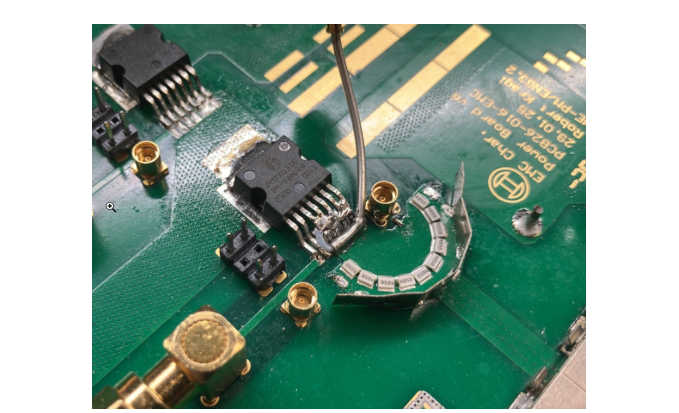
\includegraphics[scale=1]{figures/5_CurrentProbe/Diss_Pic_PShunt.pdf}
	\caption{Realization of the passive shunt for verification.}\label{fig:Diss_Pic_PShunt}
\end{figure}

As a reference, a high-ohmic shunt with \SI{250}{m\Omega} is used.
Its transfer function is shown in \fref{fig:VNA_PShunt}, where it exhibits a \mi{f}{3dB} bandwidth of \SI{385}{MHz}, which is sufficient for the low-pass verification.
The shunts are placed in the commutation loop by replacing the D2PAK source connectors with SMD shunts, while a semi-rigid coaxial SMA cable is used as the pick-up.
A photograph of the setup is shown in \fref{fig:Diss_Pic_PShunt}.

\begin{figure}[ht]
	\centering
	\input{"figures/5_CurrentProbe/VNA_PShunt.tex"}
	\caption{VNA measurement of \SI{250}{m\Omega} passive shunt.}\label{fig:VNA_PShunt}
\end{figure}


The measured current waveforms for a classical double-pulse test are shown in \fref{fig:MS_Current_AvsPShunt_TD}, comparing the low-pass of the active shunt with the passive shunt.
In addition, the common-mode error of the active shunt is plotted.
It is obtained by connecting both inputs of the active shunt to the same source potential, which should ideally produce zero output.

\begin{figure}[ht]
	\centering
	\tikzsetnextfilename{MS_Current_AvsPShunt_TD}
	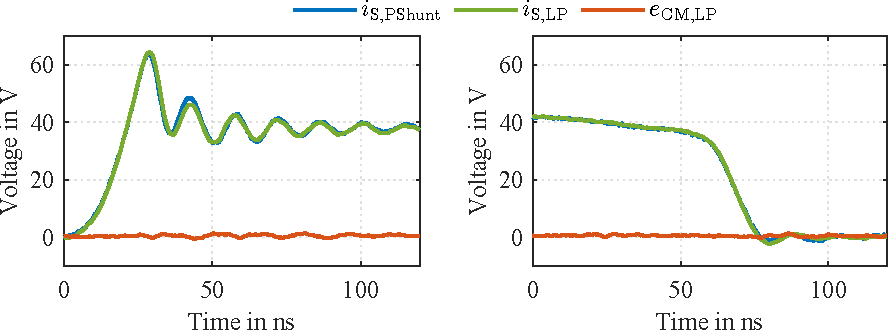
\includegraphics[scale=1]{figures/5_CurrentProbe/MS_Current_AvsPShunt_TD.pdf}
	\caption{Time-domain verification using a passive shunt.}\label{fig:MS_Current_AvsPShunt_TD}
\end{figure}

The measured waveforms show very good agreement between the active and passive shunts, both in the transient slope and in the observed overvoltage.
Only a small deviation appears in the second period of the main oscillation.
This deviation cannot be attributed to common-mode error, which is clearly much smaller.
It is therefore most likely caused by residual capacitive coupling from the voltage transient into the current shunt.


To determine how much the shield of the probe influences the measurement, a measurement with and without the shield is performed, the results of which are shown in \fref{fig:Influence_Current_Shield_TD} and \fref{fig:Influence_Current_Shield_FD}.
The influence of the capacitive coupling is barely visible in the time domain, where the unshielded measurement shows only a slightly higher overshoot and ringing.
However, when the frequency domain is considered, high differences in the two measurements can be seen.
This indicates that the shield mainly shields the high-pass path of the active shunt, which is more sensitive to coupling due to smaller signals and higher gains.

\begin{figure}[ht]
	\centering
	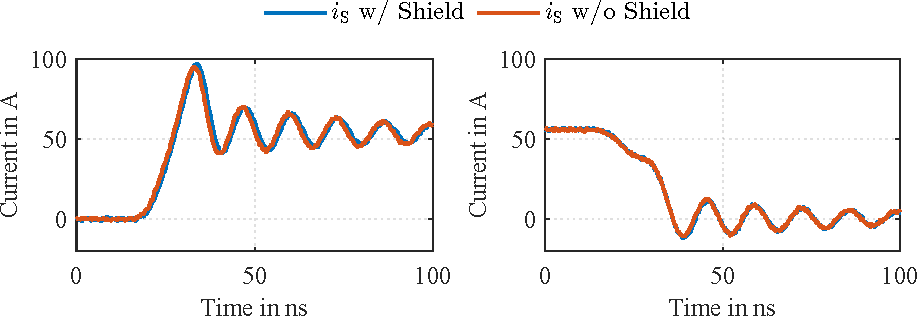
\includegraphics[scale=1]{figures/5_CurrentProbe/Influence_Shield_TD.pdf}
	\caption{Time-domain measurement results of PMTX05, at 800V, 30A room temperature, influence of the shield on the measurement.}\label{fig:Influence_Current_Shield_TD}
\end{figure}

\begin{figure}[ht]
	\centering
	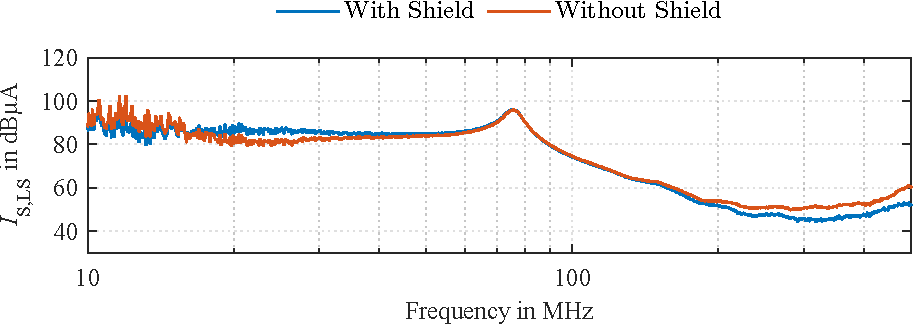
\includegraphics[scale=1]{figures/5_CurrentProbe/Influence_Shield_FD.pdf}
	\caption{Frequency-domain measurement results of PMTX05, at 800V, 30A room temperature, influence of the shield on the measurement.}\label{fig:Influence_Current_Shield_FD}
\end{figure}

\textbf{Noise Performance Characterization:}
The final step of this section is not a strict verification, but rather a characterization of the shunt's noise behavior.
This analysis is important because the active current shunt combines a low-pass path optimized for the switching waveform with a high-pass path intended to resolve the commutation transient.
The key question is therefore whether the additional gain and bandwidth of the active path raise the noise floor in a way that degrades the measurement of either the low-frequency current waveform or the high-frequency current spike.

Figure~\ref{fig:MS_Current_Noise} shows the frequency-domain noise of the active shunt for an acquisition length corresponding to the pulse-train duration used later in the measurement campaign.
To separate probe noise from the oscilloscope contribution, the measurement is performed for four conditions: the active shunt at the oscilloscope resolution used for subsequent signal measurements, the oscilloscope alone at the same resolution, the active shunt with full ADC resolution, and the oscilloscope alone with full ADC resolution.
This decomposition makes it possible to distinguish the intrinsic probe-noise floor from the quantization-noise floor of the acquisition system.

In the low-frequency range, the observed noise is dominated by the oscilloscope quantization floor.
With increasing frequency, however, the active shunt exhibits a gradual rise in noise that follows the gain characteristic of the high-pass channel.
This behavior is consistent with the principle already discussed for the voltage probe: the high-pass path amplifies both the desired signal and the input-referred noise, so the noise floor follows the slope of the transfer function.
However, because the shunt amplifiers provide higher gain than the voltage-probe stage, the thermal noise of the operational amplifiers becomes dominant over the oscilloscope quantization noise at a lower frequency, namely around \SI{120}{MHz} instead of \SI{220}{MHz}. 

\begin{figure}[hbt]
	\centering
	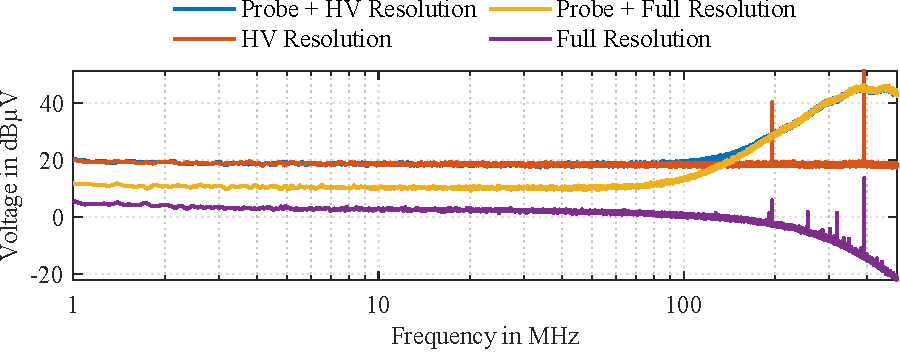
\includegraphics[scale=1]{figures/5_CurrentProbe/Diss_Current_NoiseContribution.pdf}
	\caption{Frequency-domain measurement of the noise behavior of the high-pass of the active current shunt.}\label{fig:MS_Current_Noise}
\end{figure}



\section{Measurement Environment}
\label{sec:Environment}

The measurement platform aims to incorporate the discussed sensors into a classical power electronic application, while enabling the realization of the different measurement methoodologies for the the intrinsic EM emissions of the switching device.
Furthermore, a crosscheck with classical EMC measurements, namely a LISN measurement, is deployed in the measurement environment.

A picture of the measurement setup is shown in \fref{fig:pic_b2b_setup}.

%!TeX root = main.tex
%!encoding = UTF-8 Unicode

\subsection{Requirements for the Integrated EMC Measurement Environment}

The measurement platform must fulfill several requirements to enable reproducible and EMC-relevant characterization under realistic operating conditions.
First, it must provide a classical ground reference that represents the inverter chassis and allows physically meaningful coupling paths for high-frequency currents.
Second, the switching behavior of the test setup must be comparable to that of real applications, so that the measured emission spectra remain representative of practical converter operation.
Third, the platform must support the different measurement methodologies introduced in this work, in particular the operation of pulse chains with multiple consecutive switching events at a defined operating point.
Fourth, the setup must include a conducted-EMC reference measurement based on a LISN to allow direct comparison between intrinsic device emissions and standardized system-level quantities.
Fifth, additional noise sources introduced by the test environment must be minimized.
This includes filtering of the supply paths via the LISN, optical transmission of control signals, battery-powered gate-driver supplies, and a linear load implementation based on an air-core inductor.
Finally, the platform must allow stable operation during pulse-chain measurements without requiring active thermal management; therefore, passive cooling has to be sufficient for the intended operating regime.

The design choices discussed in the following section are derived directly from these requirements and are presented in the same logical order.

%!TeX root = main.tex
%!encoding = UTF-8 Unicode

\subsection{Design of the Measurement Environment}
The measurement setup implements the instrumentation required to satisfy the requirements defined in the previous section.
Its purpose is to capture the EMC-relevant high-frequency components of the three dominant intrinsic noise contributors: the drain-source voltages of the high-side and low-side devices and the commutation-loop current.
In parallel, a conventional conducted-EMC reference measurement via line impedance stabilization networks (LISNs) is integrated.

\begin{figure}[ht]
	\centering
	\import{./figures/6_Environment/}{"Diss_Pic_Setupv5.pdf_tex"}
	\caption{Photograph of measurement environment.}\label{fig:pic_b2b_setup}
\end{figure}

The setup is shown as a photograph in \fref{fig:pic_b2b_setup}, and its equivalent circuit is depicted in \fref{fig:ESB_b2b}.
The implementation follows the requirement order given above.

To realize a classical inverter-like ground reference, the primary half-bridge with the devices under test (DUTs), \mti{Q}{LS} and \mti{Q}{HS}, is mechanically coupled to an aluminum plate.
In this setup, the plate is primarily used as a defined, low-impedance return path for high-frequency ground currents toward the LISNs, thereby reproducing a physically meaningful chassis-like reference.

To ensure application-representative switching behavior, a conventional layout derived from an on-board charger is used.
This layout yields a commutation-loop inductance of \mi{L}{\sigma} = \SI{26}{nH}, which is comparatively high relative to state-of-the-art commutation loops based on purely coplanar designs.
However, the objective of this work is not to optimize the commutation loop itself, but to characterize the intrinsic emissions of the switching device under the given parasitic conditions.

To enable pulse-chain operation for thermal-noise reduction, a back-to-back converter topology is employed, in which both half-bridges share a common DC link and are separated by the main filters of the LISNs.
This architecture allows repeated switching events to be generated at nearly identical operating conditions, thereby improving repeatability and increasing the statistical robustness of the derived frequency-domain spectra.

\begin{figure}[ht]
	\centering
	\import{./figures/6_Environment/}{"Diss_ESB_B2B.pdf_tex"}
	\caption{Equivalent circuit diagram of the back-to-back converter measurement setup.}\label{fig:ESB_b2b}
\end{figure}



To include a standardized conducted-EMC reference, both converter sides are connected via LISNs.
This enables direct comparison between intrinsic terminal quantities and system-level conducted-noise metrics.
Since the focus of this dissertation is the direct characterization of intrinsic emissions, the detailed interaction between the \mi{v}{DS} measurement and the LISN result is not discussed here; an in-depth analysis is provided in~\cite{kragl_impact_2024}.

% For this paper only the raw emissions are considered and hence, no LISNs measurements are shown.
% For an analysis of the correlation between raw emissions and system-level LISN measurement, please refer to~\cite{kragl_impact_2024}.

To suppress additional noise introduced by the environment, the secondary half-bridge is intentionally designed as a low-disturbance auxiliary stage.
It consists of \mti{Q}{LS,aux} and \mti{Q}{HS,aux}, with devices rated at twice the current of the DUTs and operated at five times the gate resistance.
This reduces the switching speed and therefore the high-frequency spectral contribution of the auxiliary branch.
In addition, the auxiliary devices are placed adjacent to, but not directly on, the aluminum plate to avoid an unintended direct coupling path into the measurement ground.

Further mitigation measures follow directly from the requirements: high-frequency isolation between the two half-bridges is established through the LISN main filters, digital control signals are transmitted via optical links, and the gate-driver supplies are battery powered.
Moreover, the load path is implemented as a linear air-core inductor to avoid nonlinear magnetic behavior that could distort the measured spectral content.

Finally, thermal operation is constrained to a regime in which passive cooling remains sufficient during pulse-chain measurements.

